\documentclass{article}[12pt]
\usepackage{physics}
\usepackage{setspace}
\usepackage{amsmath}
\usepackage{mathrsfs}
\usepackage{amssymb}
\usepackage{feynmp-auto}
\usepackage{tgtermes}
\usepackage{graphicx}
\usepackage{booktabs}
\usepackage{array}
\usepackage{caption}
\usepackage{listings}
\usepackage{xcolor}
\usepackage{helvet}
\definecolor{codegreen}{rgb}{0,0.6,0}
\definecolor{codegray}{rgb}{0.5,0.5,0.5}
\definecolor{codepurple}{rgb}{0.58,0,0.82}
\definecolor{backcolour}{rgb}{0.95,0.95,0.92}
\definecolor{lightgray}{rgb}{0.95,0.95,0.95}

\lstdefinestyle{mystyle}{
    backgroundcolor=\color{lightgray},   
    commentstyle=\color{codegreen},
    keywordstyle=\color{magenta},
    numberstyle=\tiny\color{codegray},
    stringstyle=\color{codepurple},
    basicstyle=\fontfamily{pcr}\selectfont\footnotesize,
    breakatwhitespace=false,         
    breaklines=true,                 
    captionpos=b,                    
    keepspaces=true,                 
    numbers=left,                    
    numbersep=5pt,                  
    showspaces=false,                
    showstringspaces=false,
    showtabs=false,                  
    tabsize=2
}
\setcounter{page}{23}
\setcounter{figure}{10}
\setcounter{table}{1}
\lstset{style=mystyle}
\captionsetup{font=footnotesize}
\newcommand{\RN}[1]{%s
  \textup{\uppercase\expandafter{\romannumeral#1}}%
}
\usepackage{geometry}
\geometry{
 a4paper,
 left=25.4mm,
 right=25.4mm,
 top=30mm,
 bottom=25.4mm
 }
\begin{document}
\section*{5. Result}
\begin{spacing}{1.5}
\subsection*{5.1 Summary}
  To investigate the physical changes occurring in the Josephson junction based on the results of the previous sections, 
  we used two methods to analyze the calculation result. The first involved examining the changes in the order parameter, $\cos{\phi}$. 
  As a second method, we calculate the correlation function between the excited and ground states, 
  and express it using an approximation formula for conductivity based on fluctuation-dissipation theory. 
  Through analyzing the method of the order parameter, we revealed that the system exhibited an insulating state as the temperature decreased. 
  Secondly, the approximation formula showed the following results. To evaluate the accuracy of the calculated results, 
  we tested each section of the integration code by comparing it with the case without reservoir effects, 
  comparing it with higher-order approximation methods, and checking for convergence depending on the calculation conditions.
\subsection*{5.2 Benchmark}
\subsubsection*{Exact diagonalization in single mode}
To compare with the result from exact diagonalization(ED), we set the condition when the bath has only a single mode. 
The result shows approximation method could be reliable in high temperatures ($\beta = 1$).
\begin{figure}[htbp]
  \centerline{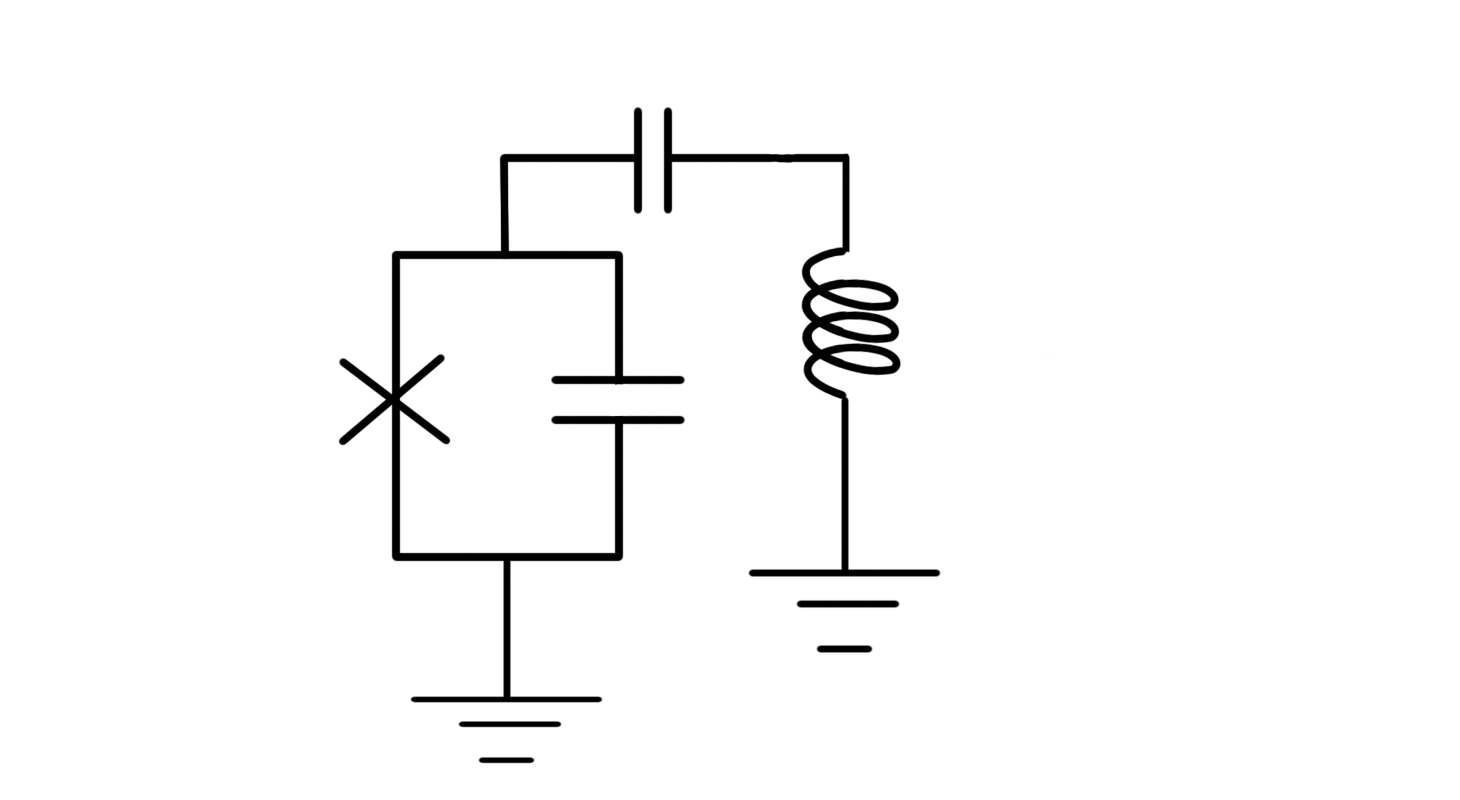
\includegraphics[width=7cm]{TexFigure/kps_singlebath.png}}
  \caption{Brief circuit scheme for single bath condition. The crossing symbol  refers to the insulated junction of Josephson junction.}
\end{figure}
\begin{figure}[htbp]
  \centerline{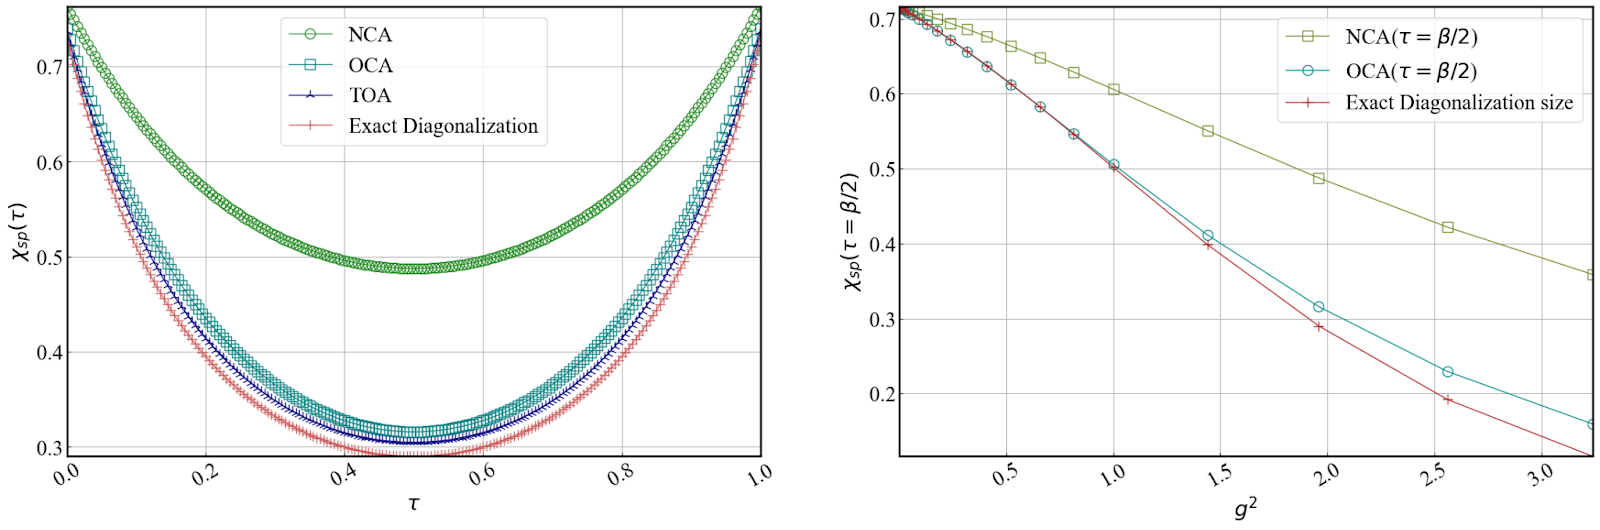
\includegraphics[width=10cm]{TexFigure/bench_single_two.png}}
  \caption{Result for single bath benchmark. For $\chi_{sp} - \tau$(Left), it conducted on overall condition g (coupling strength with system-bath) = 1.
  With $\chi_{sp}(\tau=\beta/2)-g^2$(Right), It shows that if order of perturbation increases, the results approach the exact results.}
\end{figure}
\subsubsection*{Multi-mode case}
To investigate the convergence of the diagrammatic approximation method in a general bosonic reservoir condition, 
we calculated the order parameter and the correlation function using the NCA, OCA, and TOA. 
The results showed no significant difference between the OCA and TOA calculations, confirming that the OCA is a sufficiently convergent method.
\begin{figure}[htbp]
  \centerline{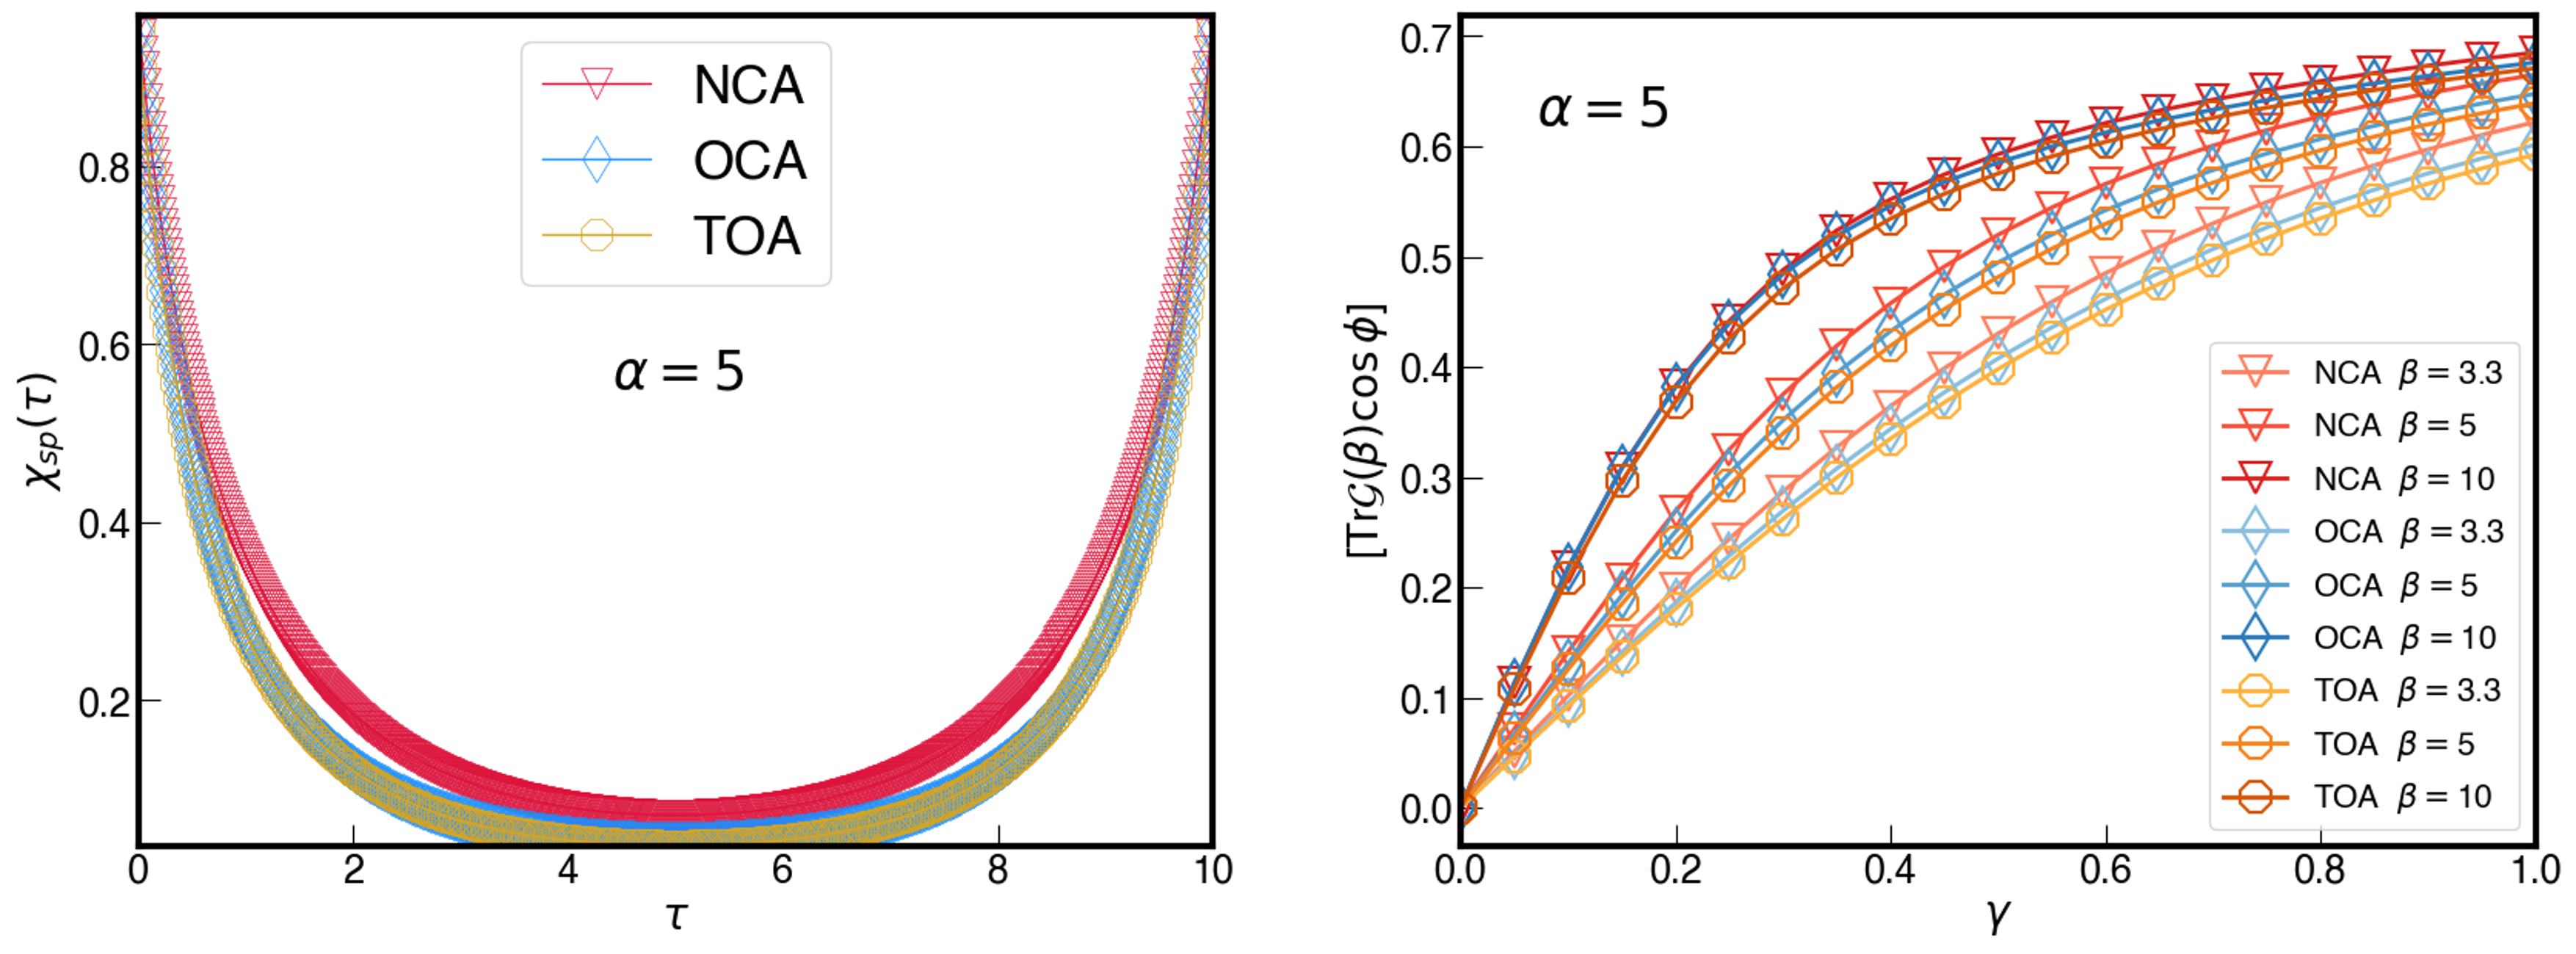
\includegraphics[width=10cm]{TexFigure/Multi_bench.png}}
  \caption{ Calculation results of the order parameter and correlation function using each order of the approximation method. 
  Both figures are for the case of $\alpha$=5, with the left figure showing temperatures between 0.3 and 0.1, 
  the right figure is for the temperature condition of 0.1. It can be observed that the calculation results of OCA and TOA are converged. 
  The size of the τ grid used for the calculation is 701.}
\end{figure}
\subsubsection*{Benchmarking solver code in $\alpha$ = 0 condition}
To check for the integration code, we compared the order parameter calculated using approximation methods for the case of α=0 
with the order parameter calculated using the state density matrix of the Josephson junction system. 
The results showed that the two cases were completely consistent.
\begin{figure}[htbp]
  \centerline{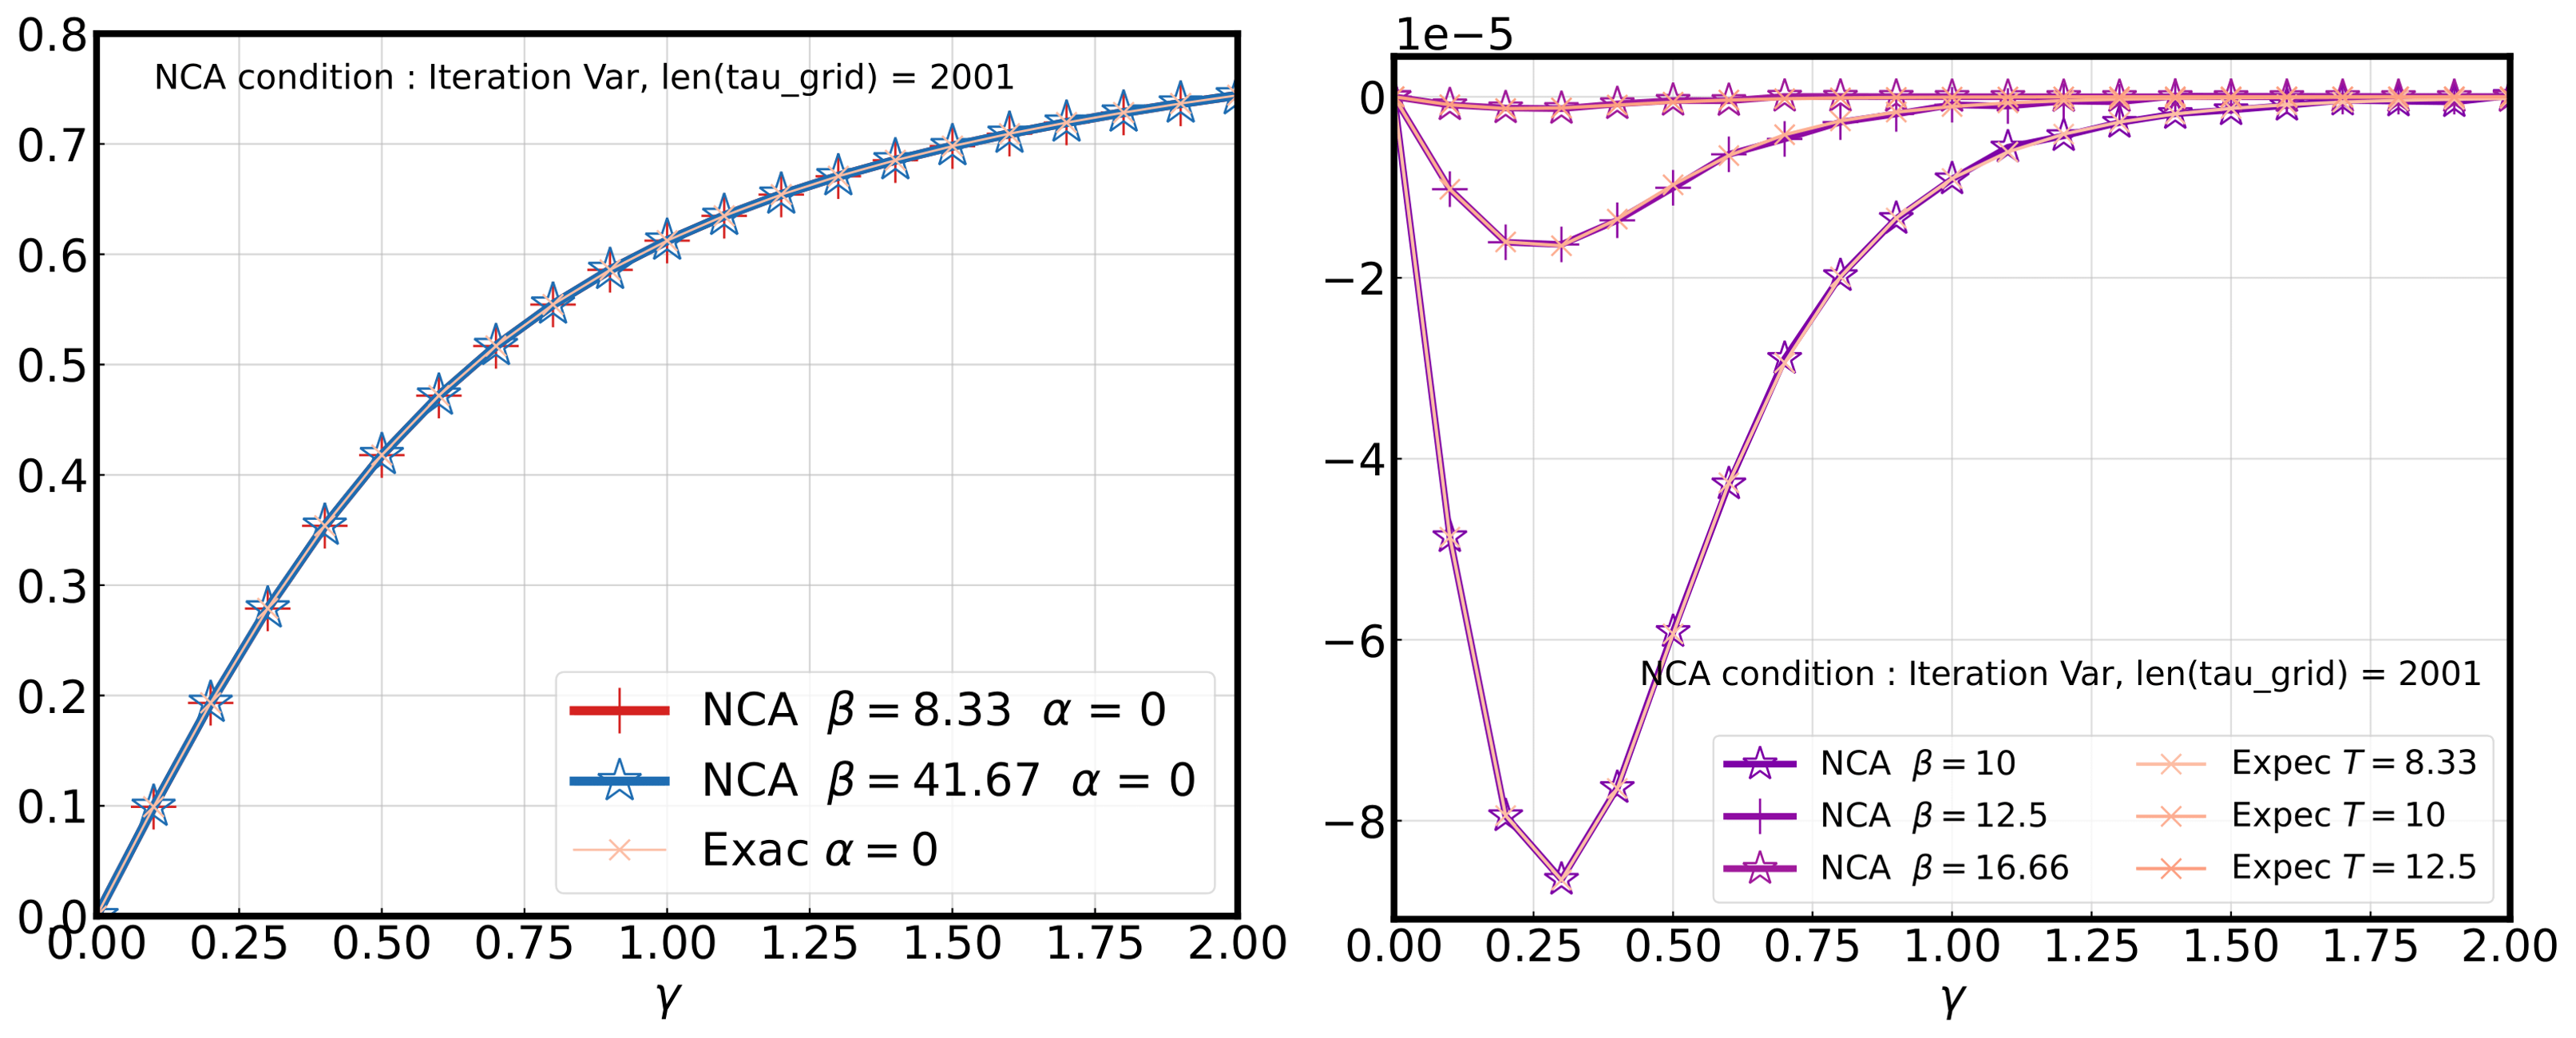
\includegraphics[width=10cm]{TexFigure/Dens_comp.png}}
  \caption{In the case of $\alpha = 0$, order parameter calculation using the approximation method should be consistent with using $H_{loc}$.
  The comparison confirmed that the two cases show consistency. The left figure shows the calculation of the order parameter, 
  and the right figure shows the difference in the order parameter for consecutive $\beta$ values,
   in the intervals [8.33, 10], [10, 12.5], and [12.5, 16.6].}
\end{figure}
\subsection*{5.3 Simulation condition}
The control parameters are as follows: $\gamma$ represents the nonlinearity of the Josephson junction system, 
$\alpha$ represents the interaction with the external environment. 
The factors influencing the accuracy of the approximation method are the number of integration iterations and the size of the $\tau$ grid. 
We set the range of variables used in the simulation as Table 2 and Table 3.
\begin{table}[htbp]
  \centering
  \renewcommand{\arraystretch}{1.2}  % 행 간격 조정
  \begin{tabular}{@{}cccc@{}}
  \toprule
  \textbf{Variables} & \textbf{Min} & \textbf{Max}  & \textbf{Interval}\\ 
  \midrule
  $\gamma$ & 0 & 2 & 0.1 \\
  $\alpha$ & 0 & 2 & 0.01 \\
  $\beta$ & 7.14 & 62.5 &  \\
  Temperature & 0.016 & 0.14 & 0.02 (until 0.04) \\
  \bottomrule
  \end{tabular}
  \caption{Parameter interval used for calculation.}
  \end{table}
\begin{table}[htbp]
  \centering
  \renewcommand{\arraystretch}{1.2}  % 행 간격 조정
  \begin{tabular}{@{}ccc@{}}
  \toprule
  \textbf{Number} & \textbf{Interval} & \textbf{Gridsize}\\ 
  \midrule
  $\tau$ grid & [0,$\beta$] & 2000 \\
  k grid & [0,K = 30000] & 30000 \\
  \bottomrule
  \end{tabular}
  \caption{Grid condition used for calculation.}
  \end{table}
\subsection*{Saturation test}
We investigated the convergence behavior of the calculation results for the change of the order parameter. 
We were able to confirm that the results converge for the case of a tau grid size of 1800 to 2000. 
\begin{figure}[htbp]
  \centerline{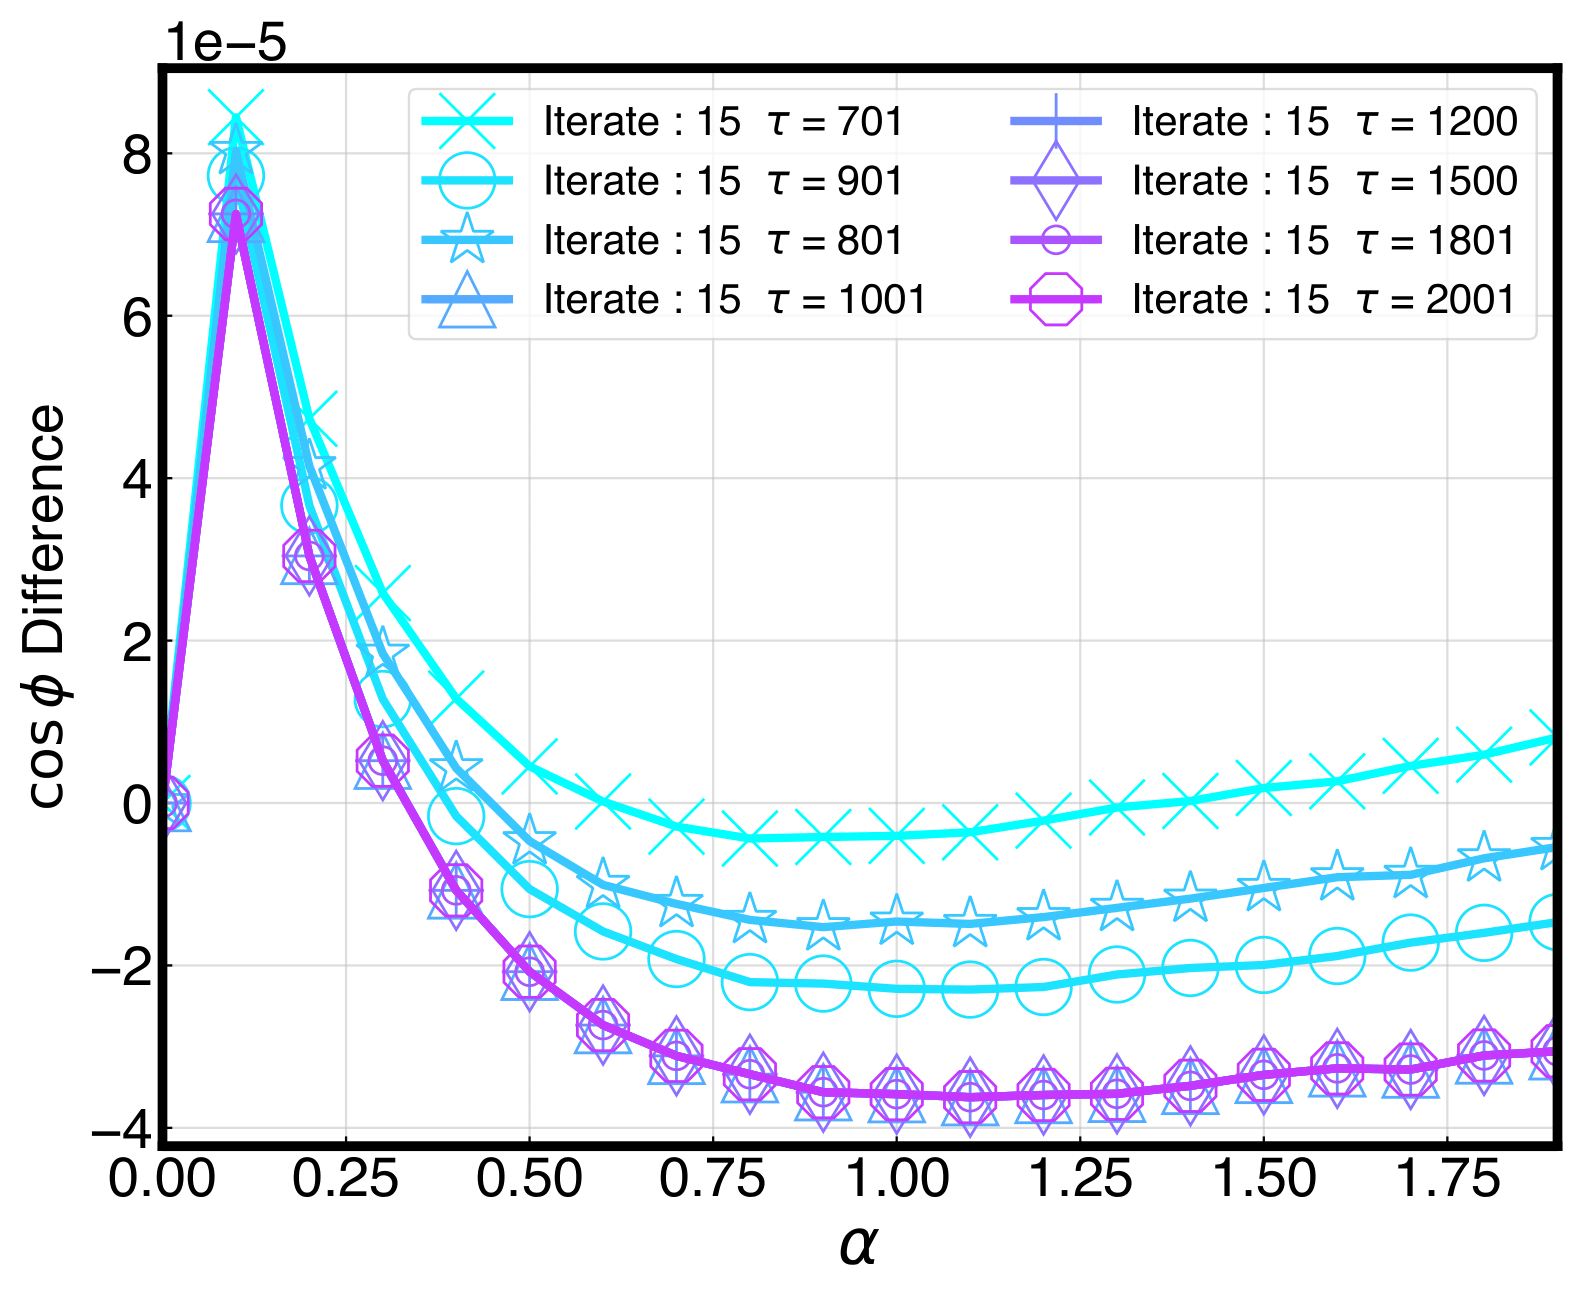
\includegraphics[width=7cm]{TexFigure/Diff_Ns3_g_b_35.71_41.67_n_15_tauchange (1)-1.png}}
  \caption{Saturation test in different time grid size. The temperature condition is $\beta = 41.67$}
\end{figure}
\subsection*{5.4 Orderparmeter}
We calculated the expectation value of the order parameter, $\cos\phi$ for various temperatures at $\alpha = 0.1$. 
In Figure 16, The results showed that the Josephson junction exhibits superconducting behavior as the nonlinearity increases at all temperatures. 
Subsequently, we examined the diagonal elements of $\cos\phi \cdot e^{−βH_{loc}}$ for $\alpha=$ 0, 0.1, and 1. 
In this case, the diagonal elements represent the system being in the ground state, the even-function form of the first excited state, 
and the odd-function form of the first excited state, respectively. 
For all cases, we confirmed that the system will localized as in the ground state. 
This indicates that the system exhibits superconductivity, consistent with the observed expectation value of the order parameter.\\
\begin{figure}[htbp]
  \centerline{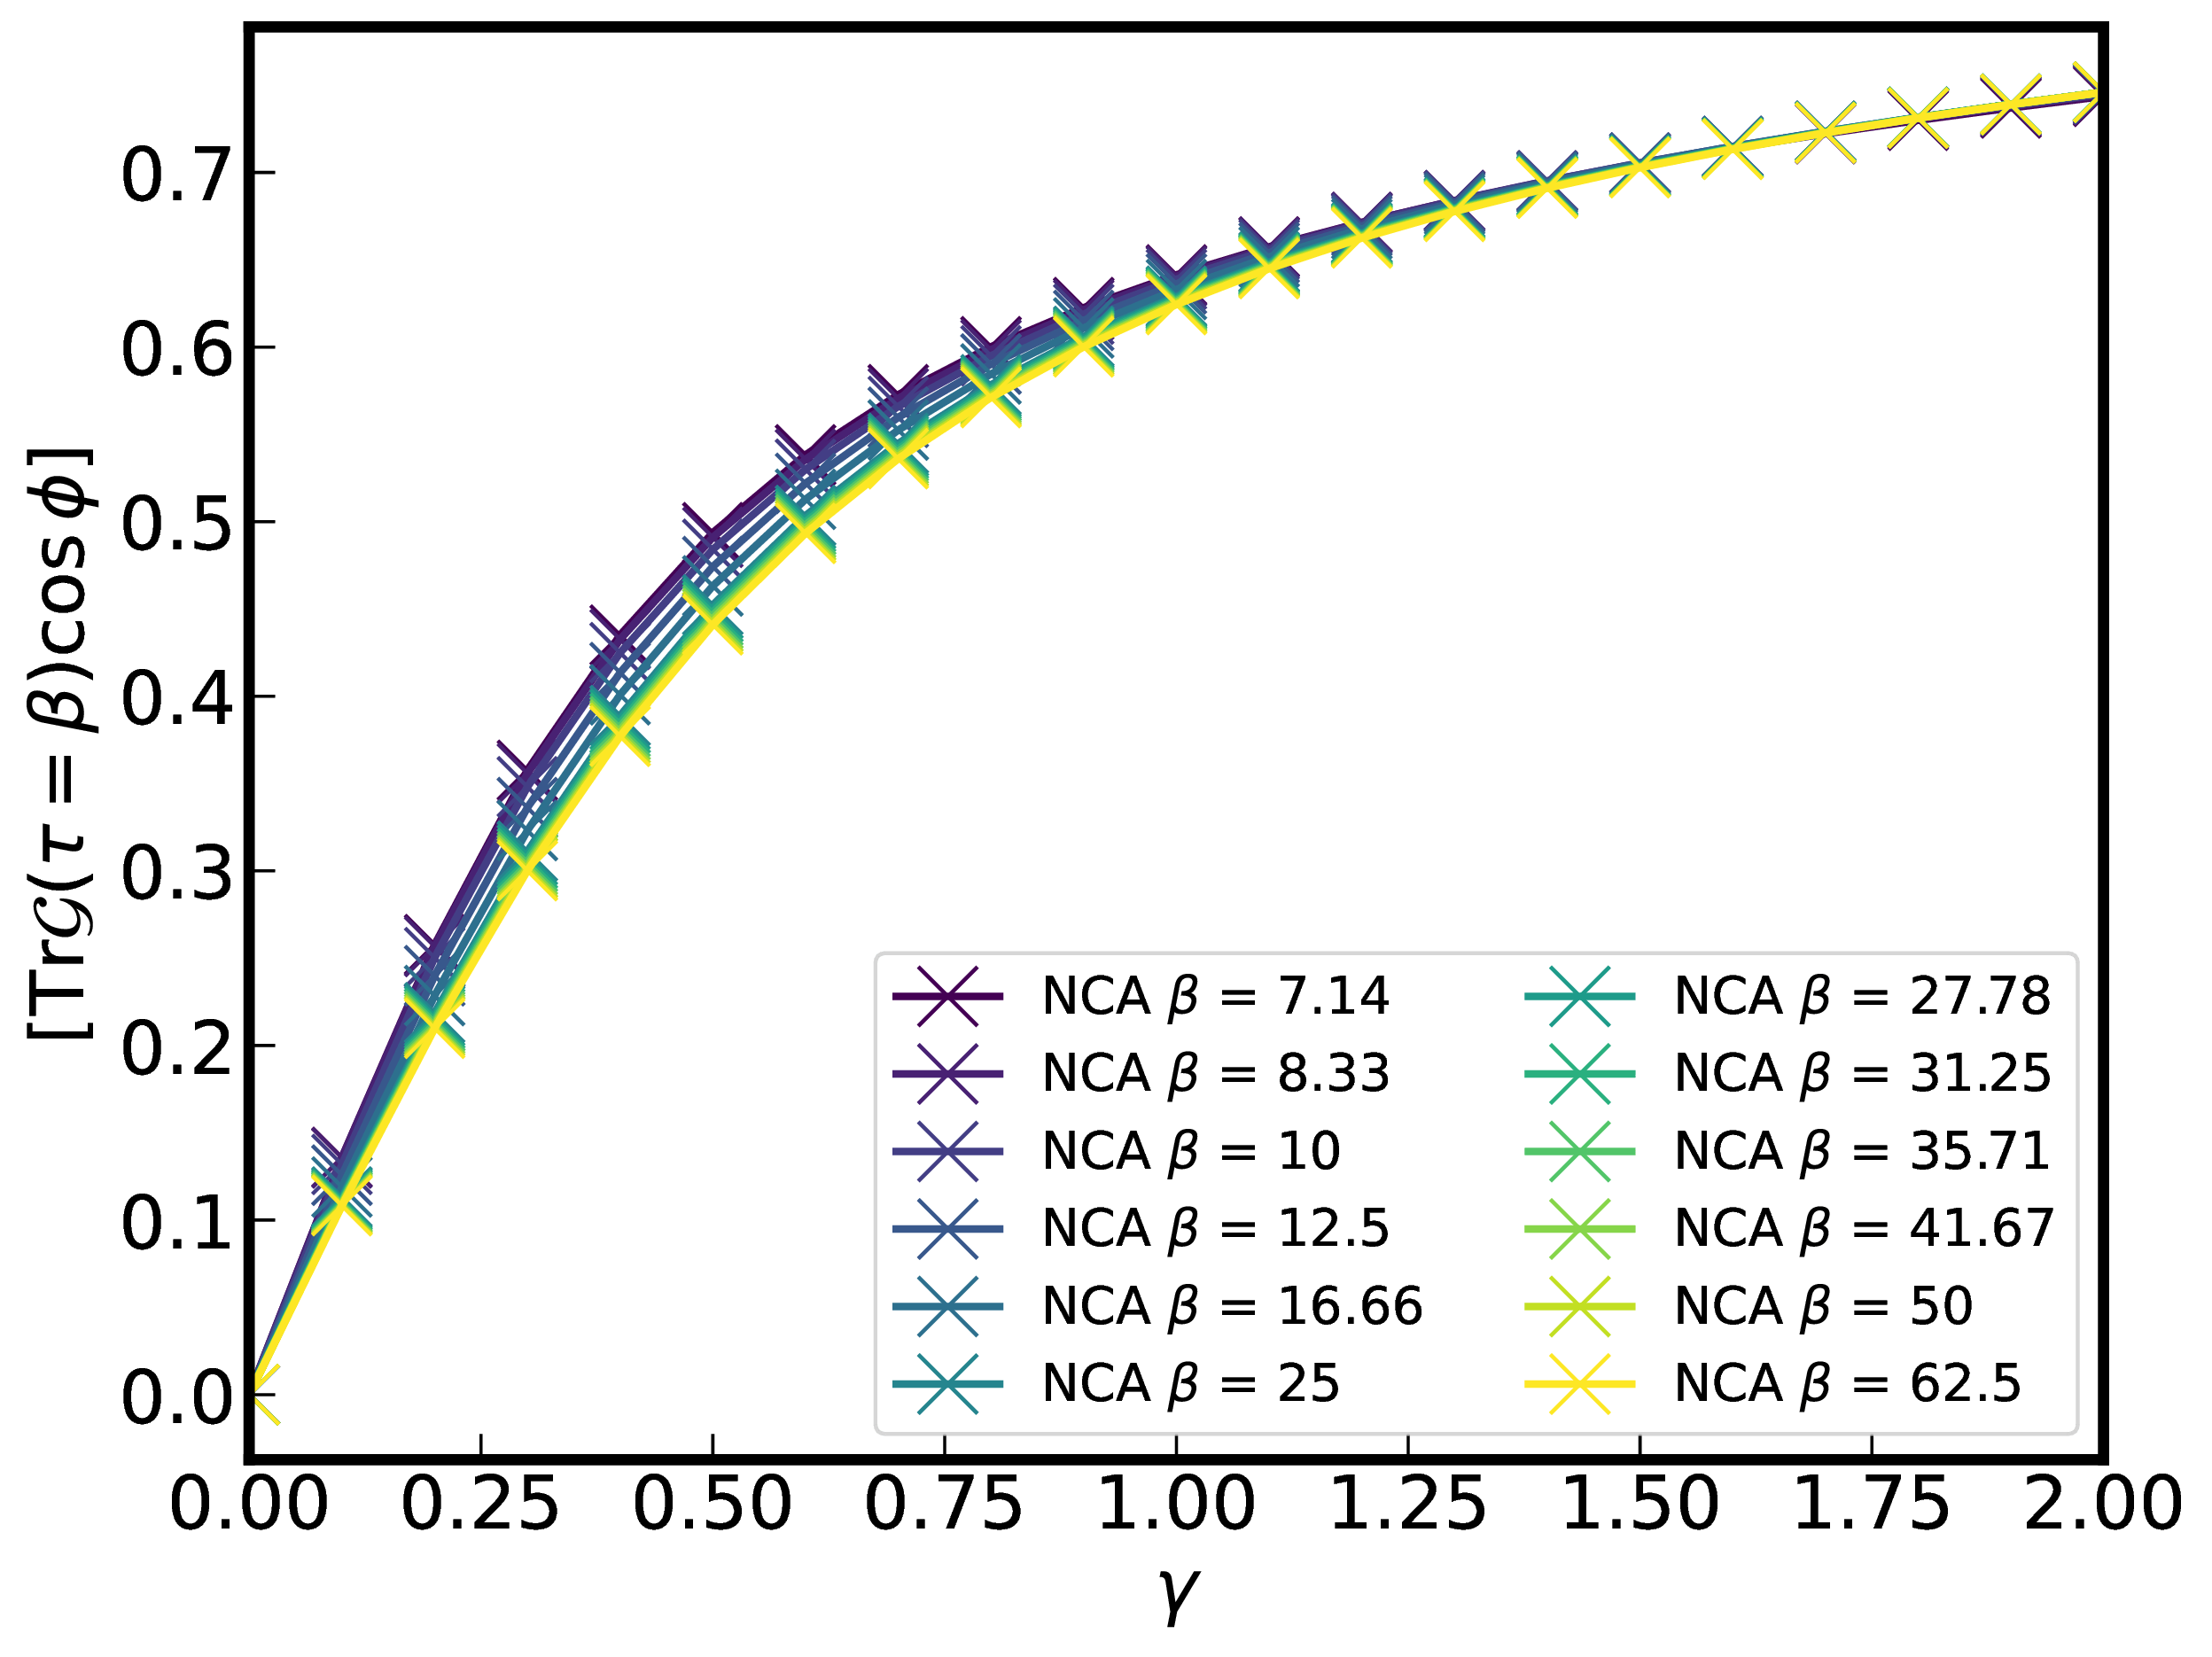
\includegraphics[width=9cm]{TexFigure/Expec_alp_0.1 (1).png}}
  \caption{Result of the expectation of order parameter, $\cos\phi$.}
\end{figure}
\begin{figure}[htbp]
  \centerline{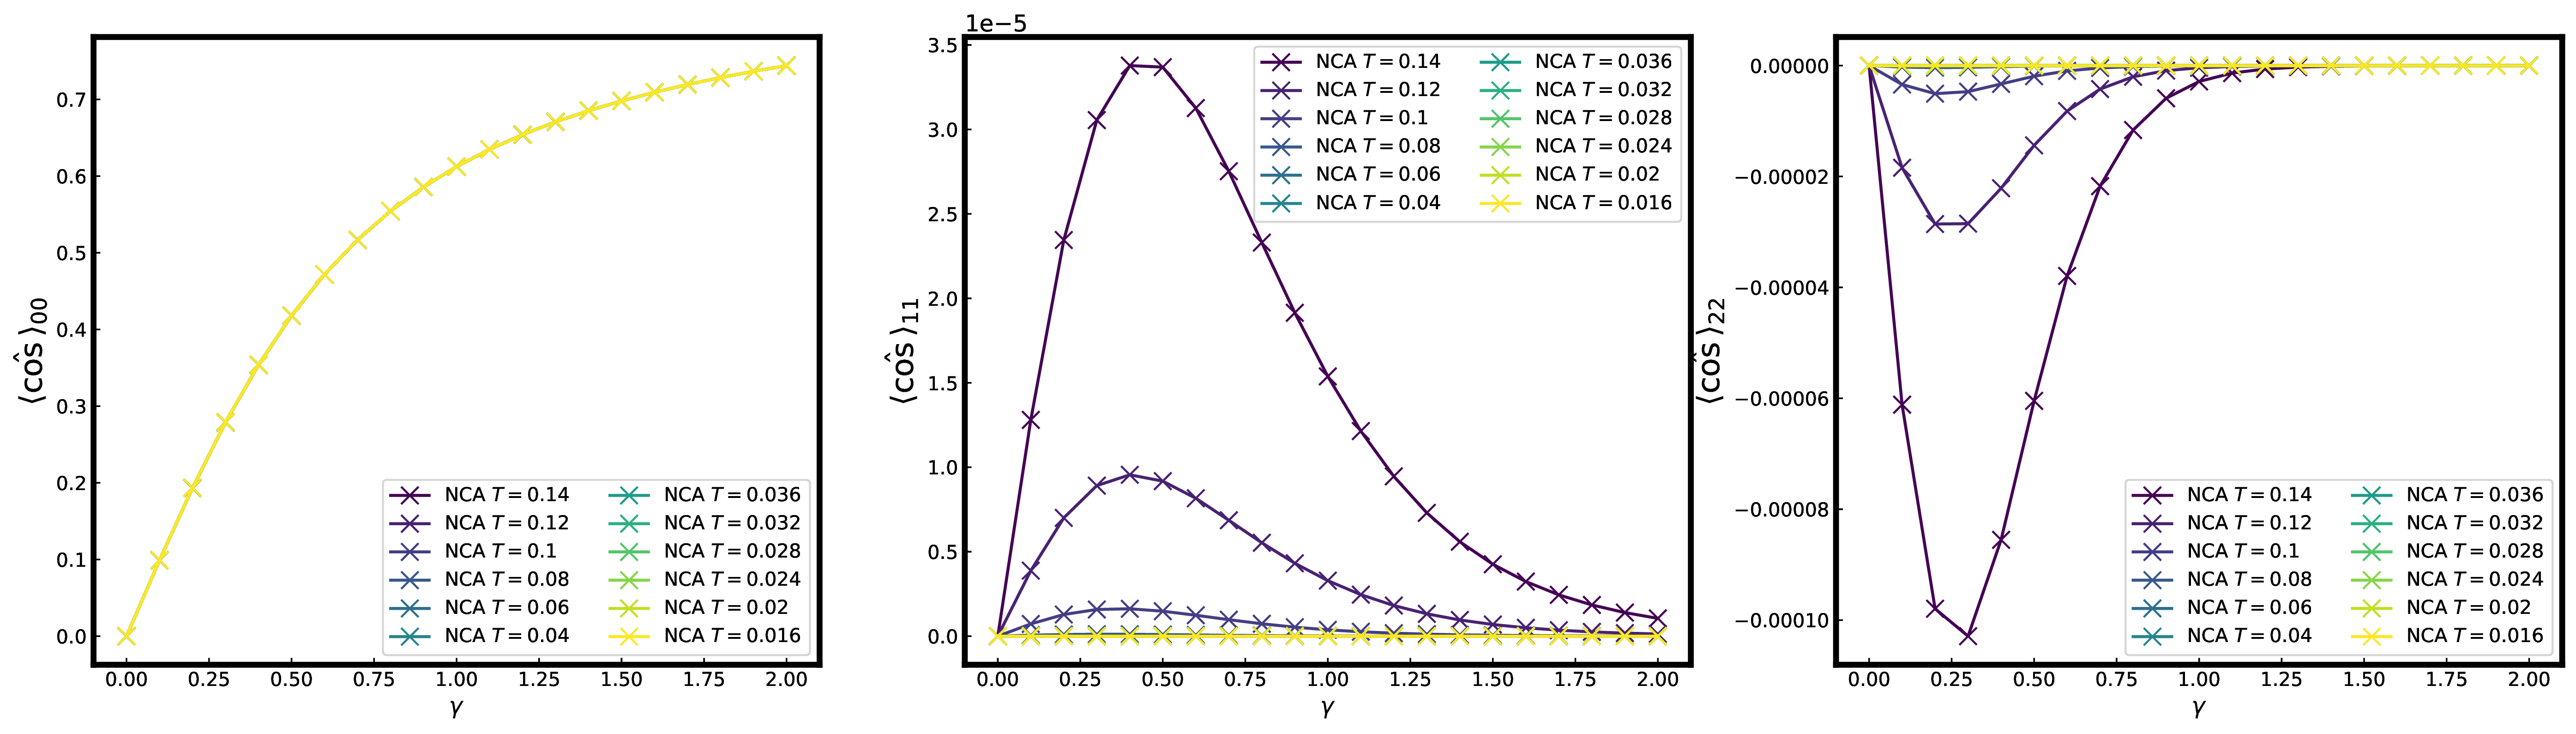
\includegraphics[width=14cm]{TexFigure/Matele_Ns3_alp0.png}}
  \centerline{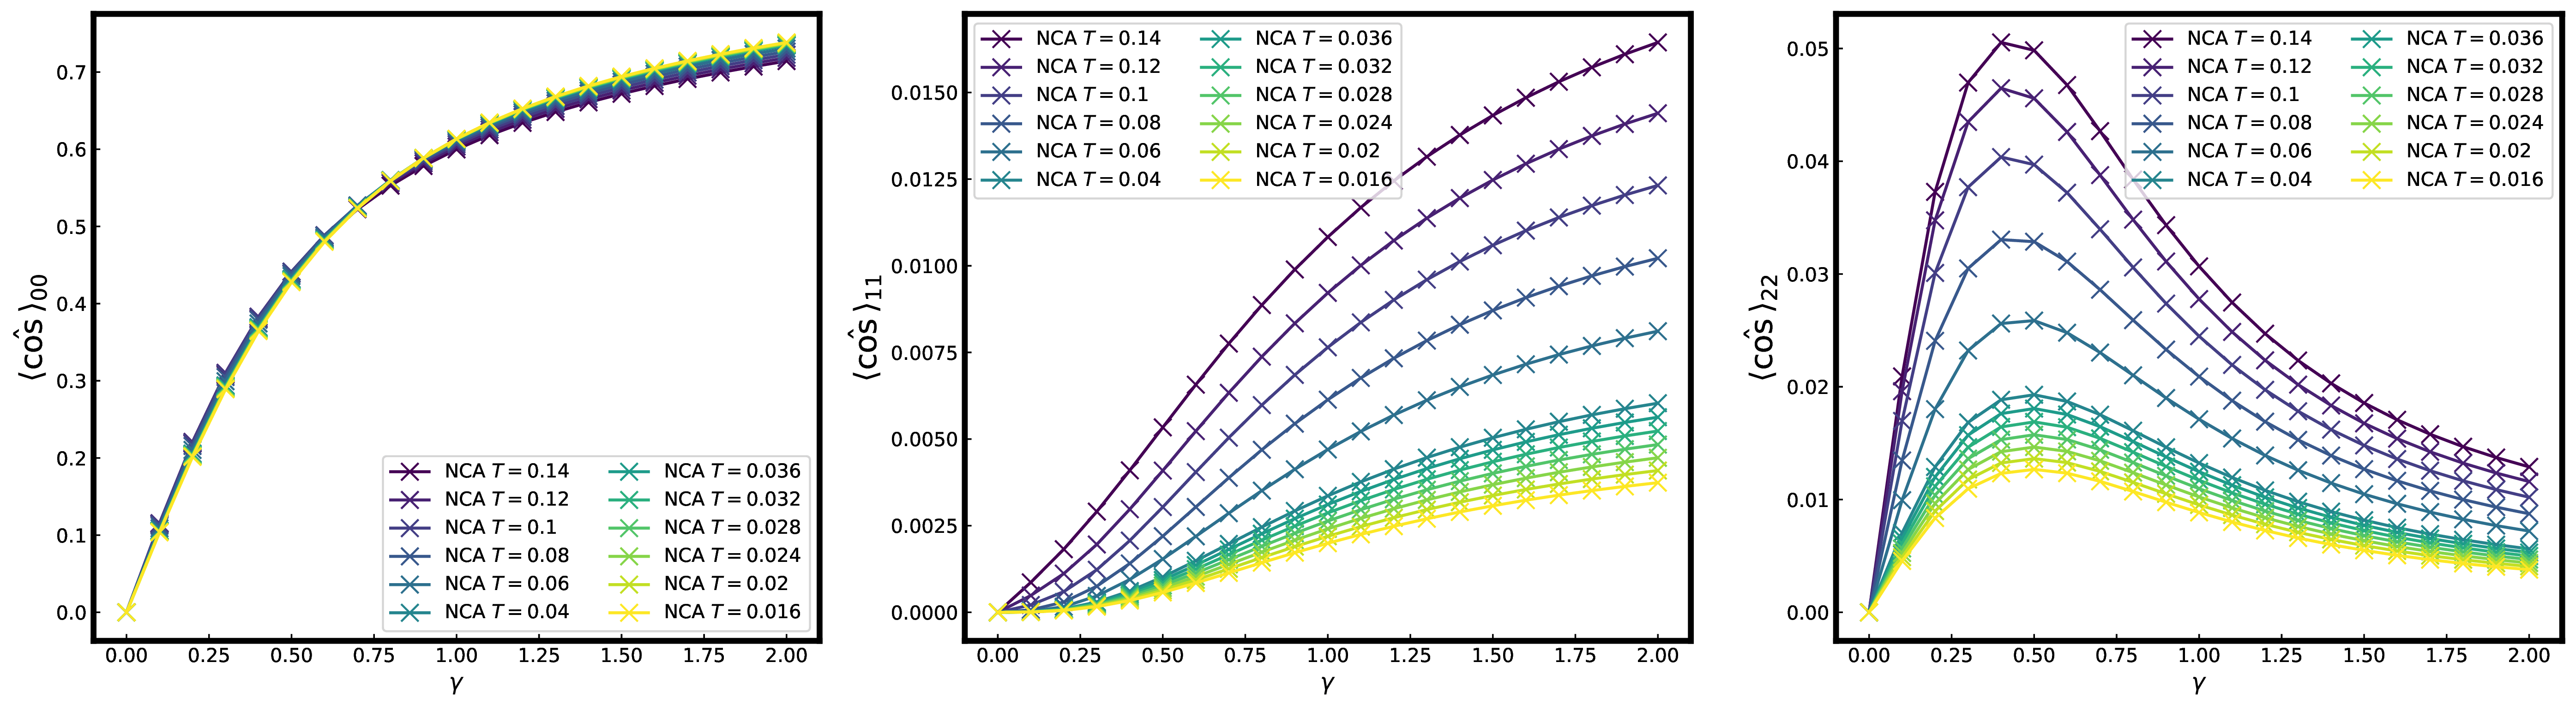
\includegraphics[width=14cm]{TexFigure/Matele_Ns3_alp0_1.png}}
  \centerline{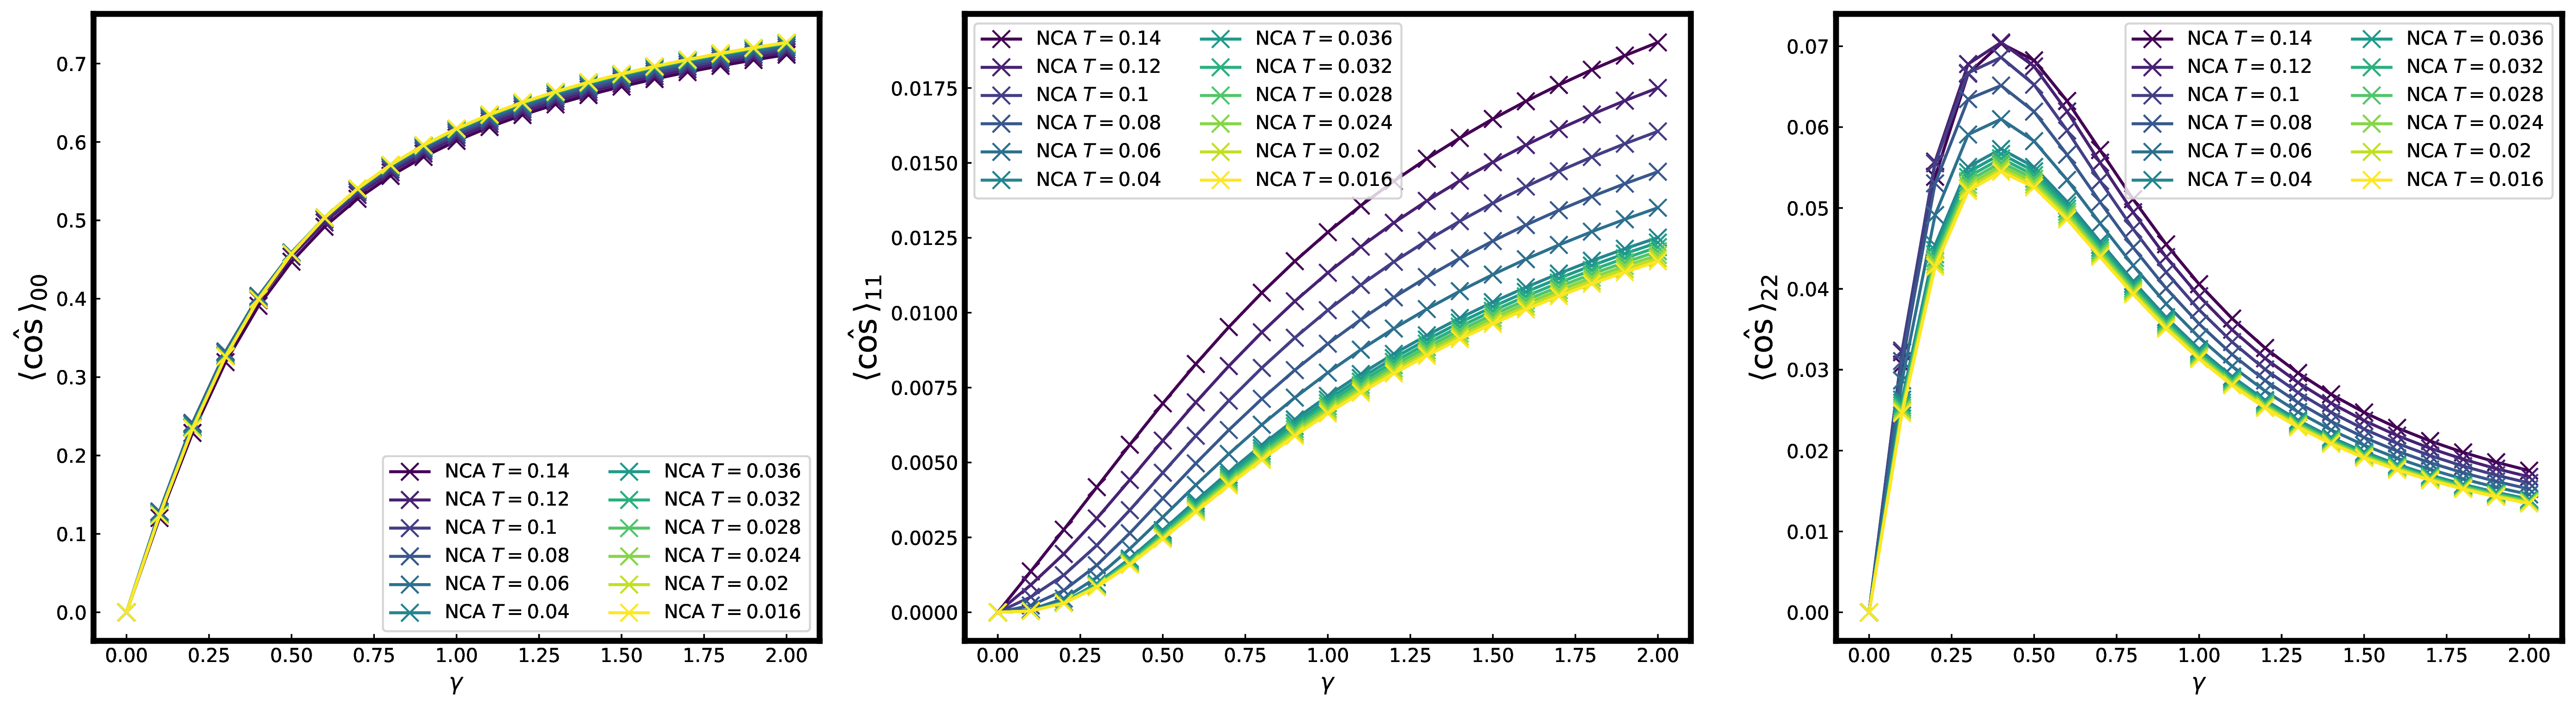
\includegraphics[width=14cm]{TexFigure/Matele_Ns3_alp1.png}}
  \caption{Change of matrix element of matrix multiplication result between $\cos\phi$ and density matrix.}
\end{figure}
\subsubsection*{Finite temperature criticality}
To confirm the criticality of the system's phase with respect to temperature, 
we observed the change in the order parameter while varying the temperature. As the temperature decreases, 
the rate of change of the order parameter shifts from a high slope to a low slope. 
It can be predicted that a temperature-dependent phase transition occurs at the given point.\\
\begin{figure}[htbp]
  \centerline{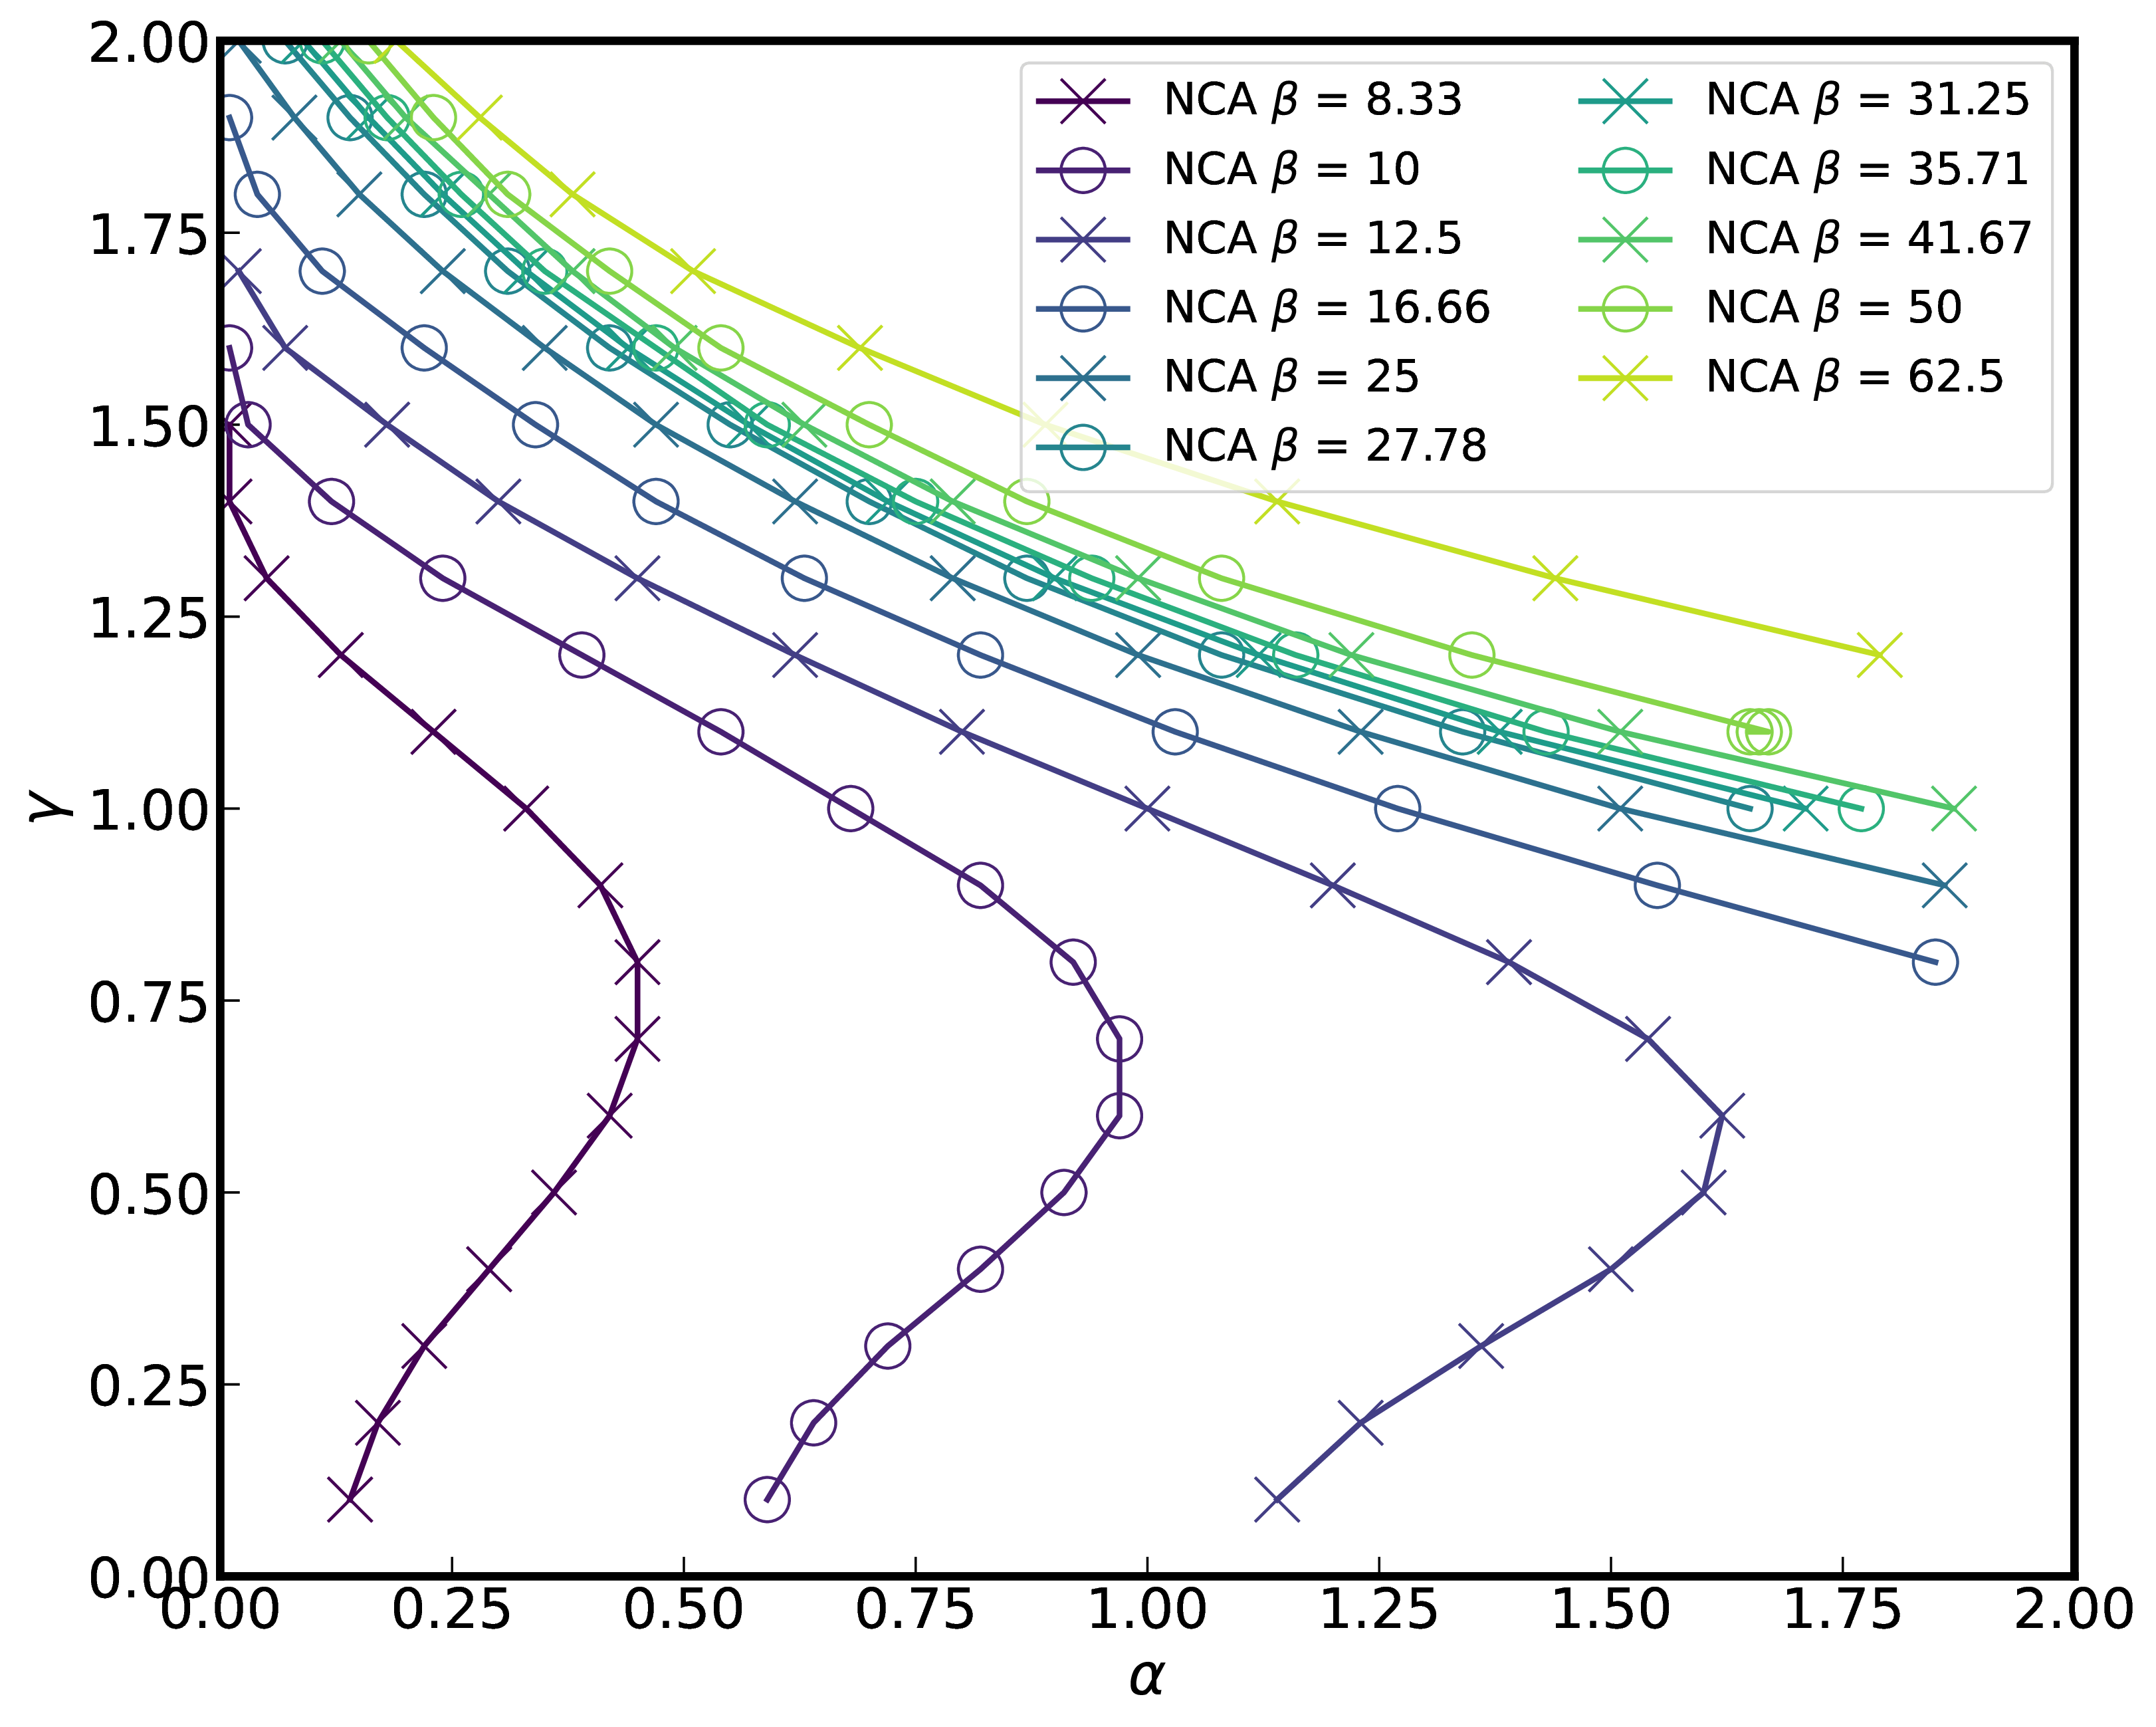
\includegraphics[width=9cm]{TexFigure/3dplot_Ns3_proj_n (2).png}}
  \centerline{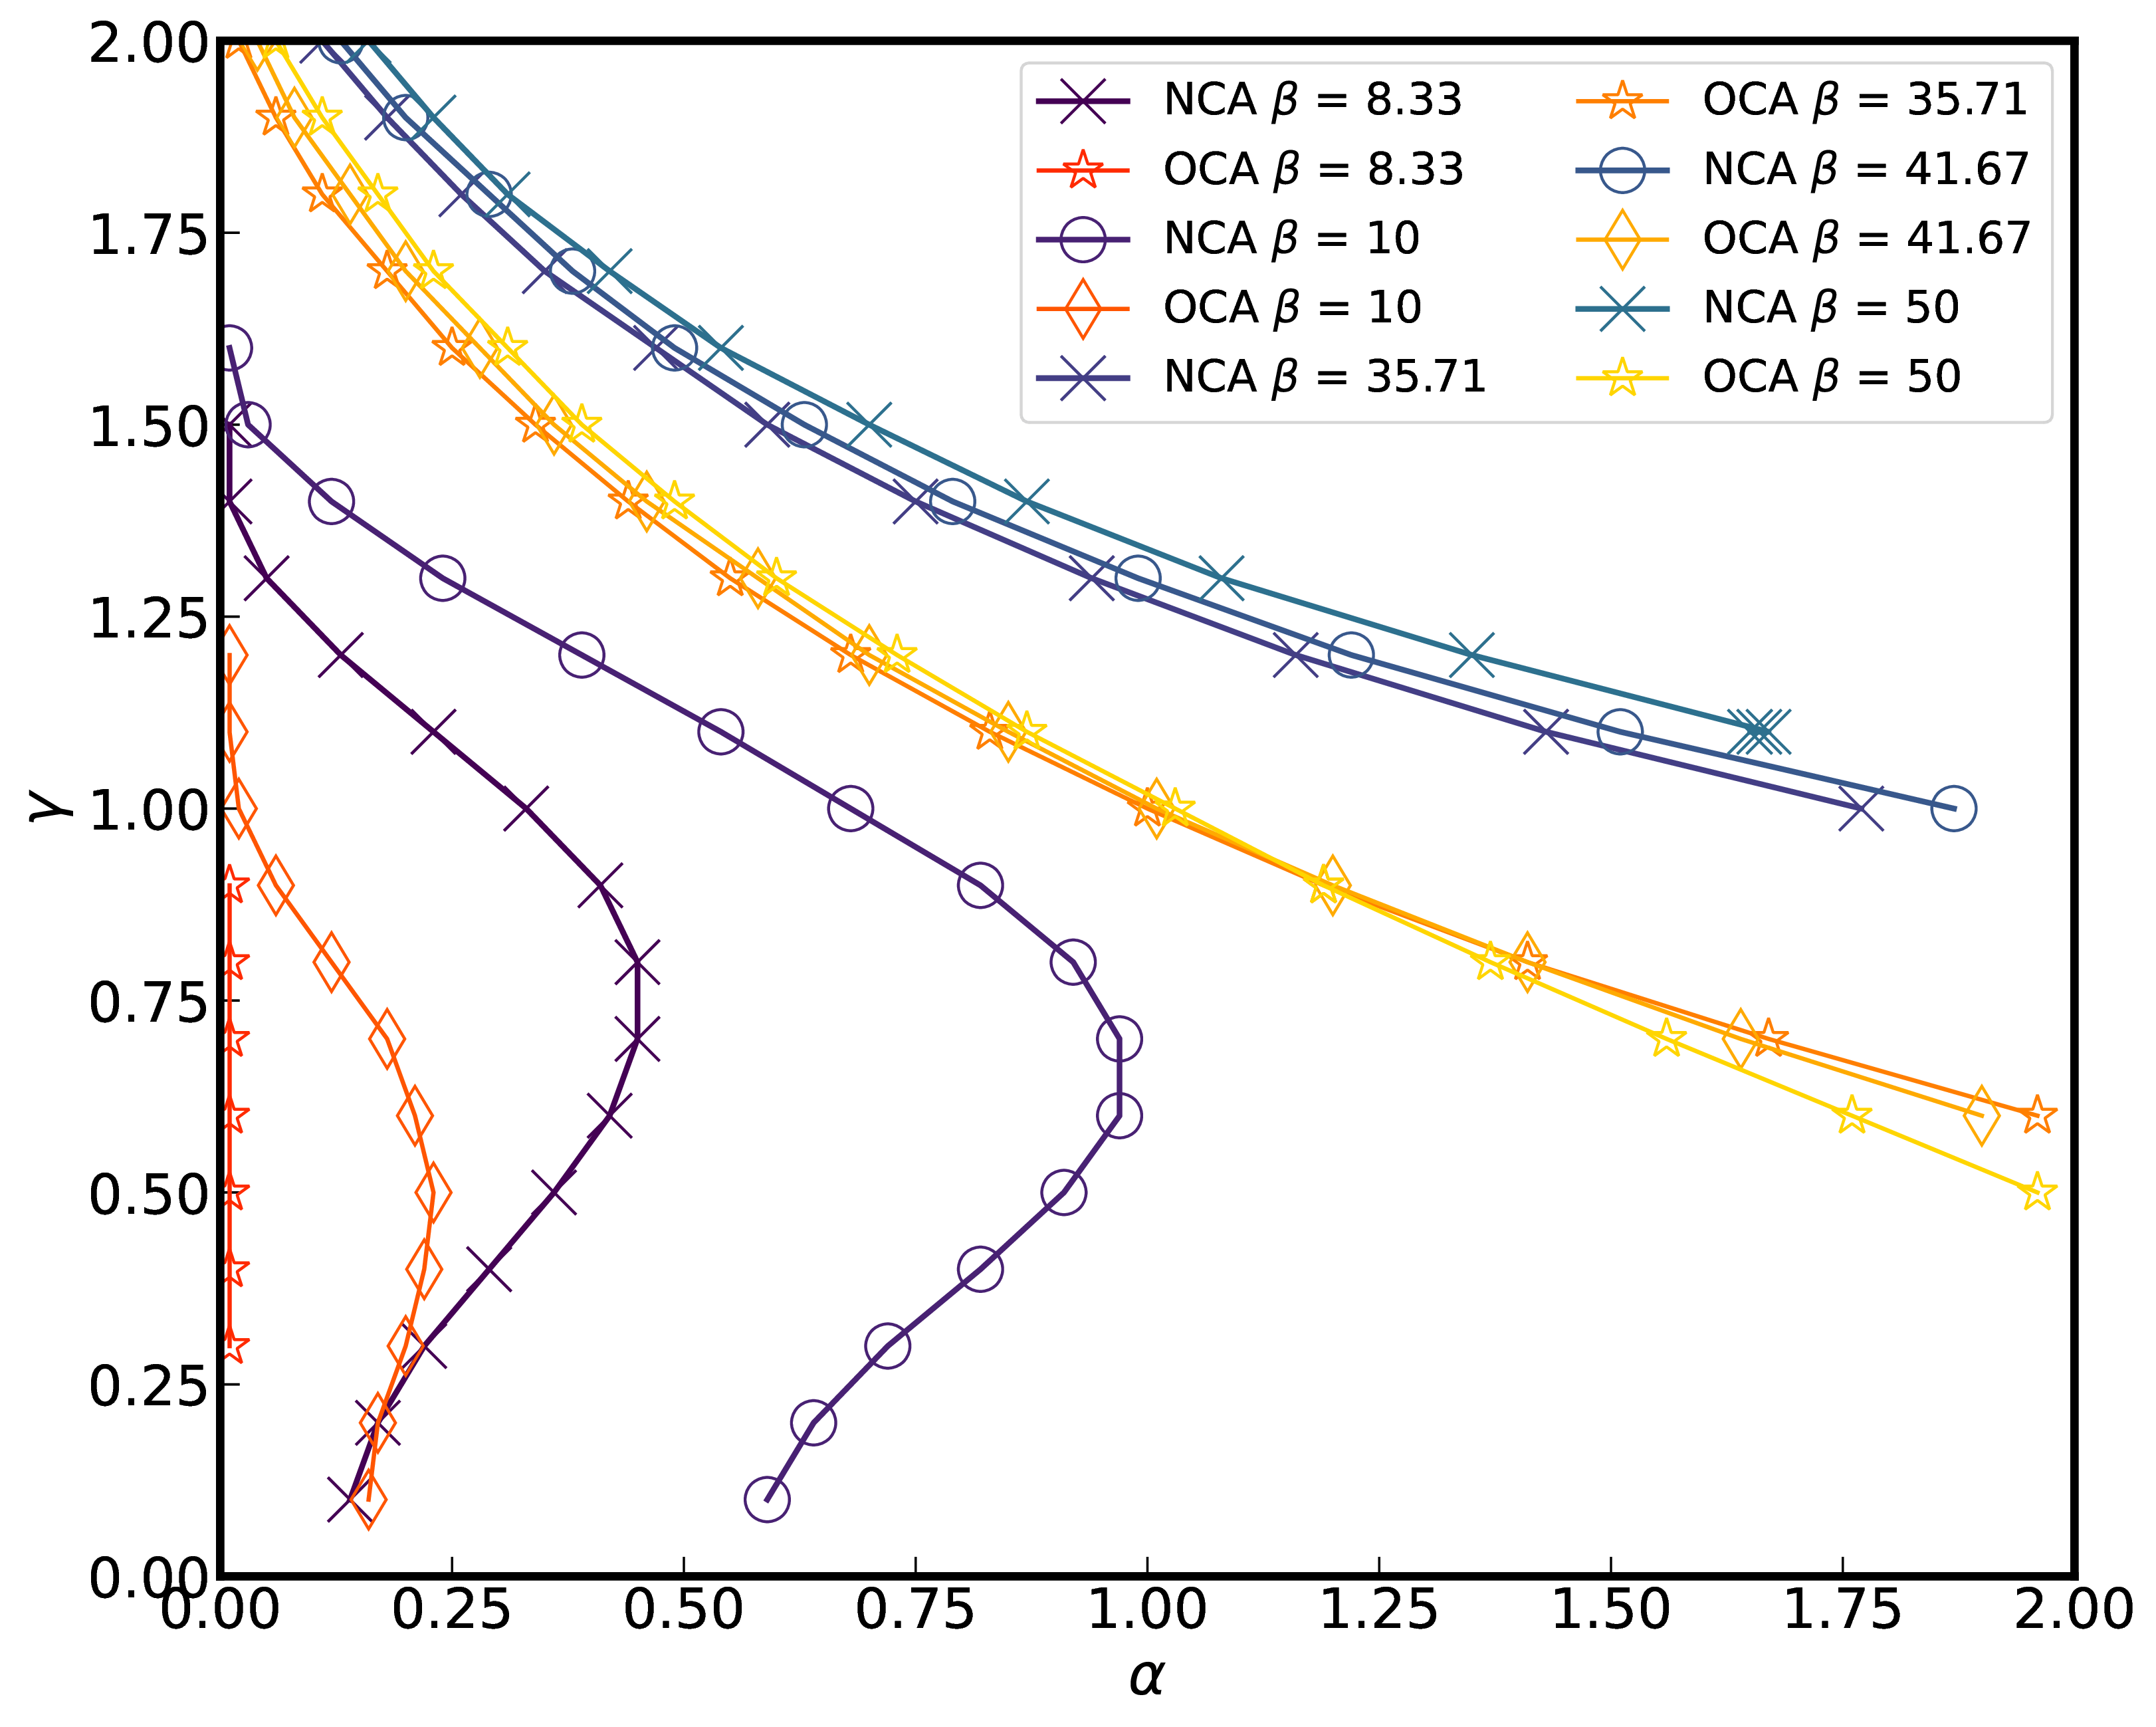
\includegraphics[width=9cm]{TexFigure/3dplot_COMP3_proj_n (2).png}}
  \caption{Finite temperature change. Figure in below is the comparision between NCA and OCA.}
\end{figure}
\begin{figure}[htbp]
  \centerline{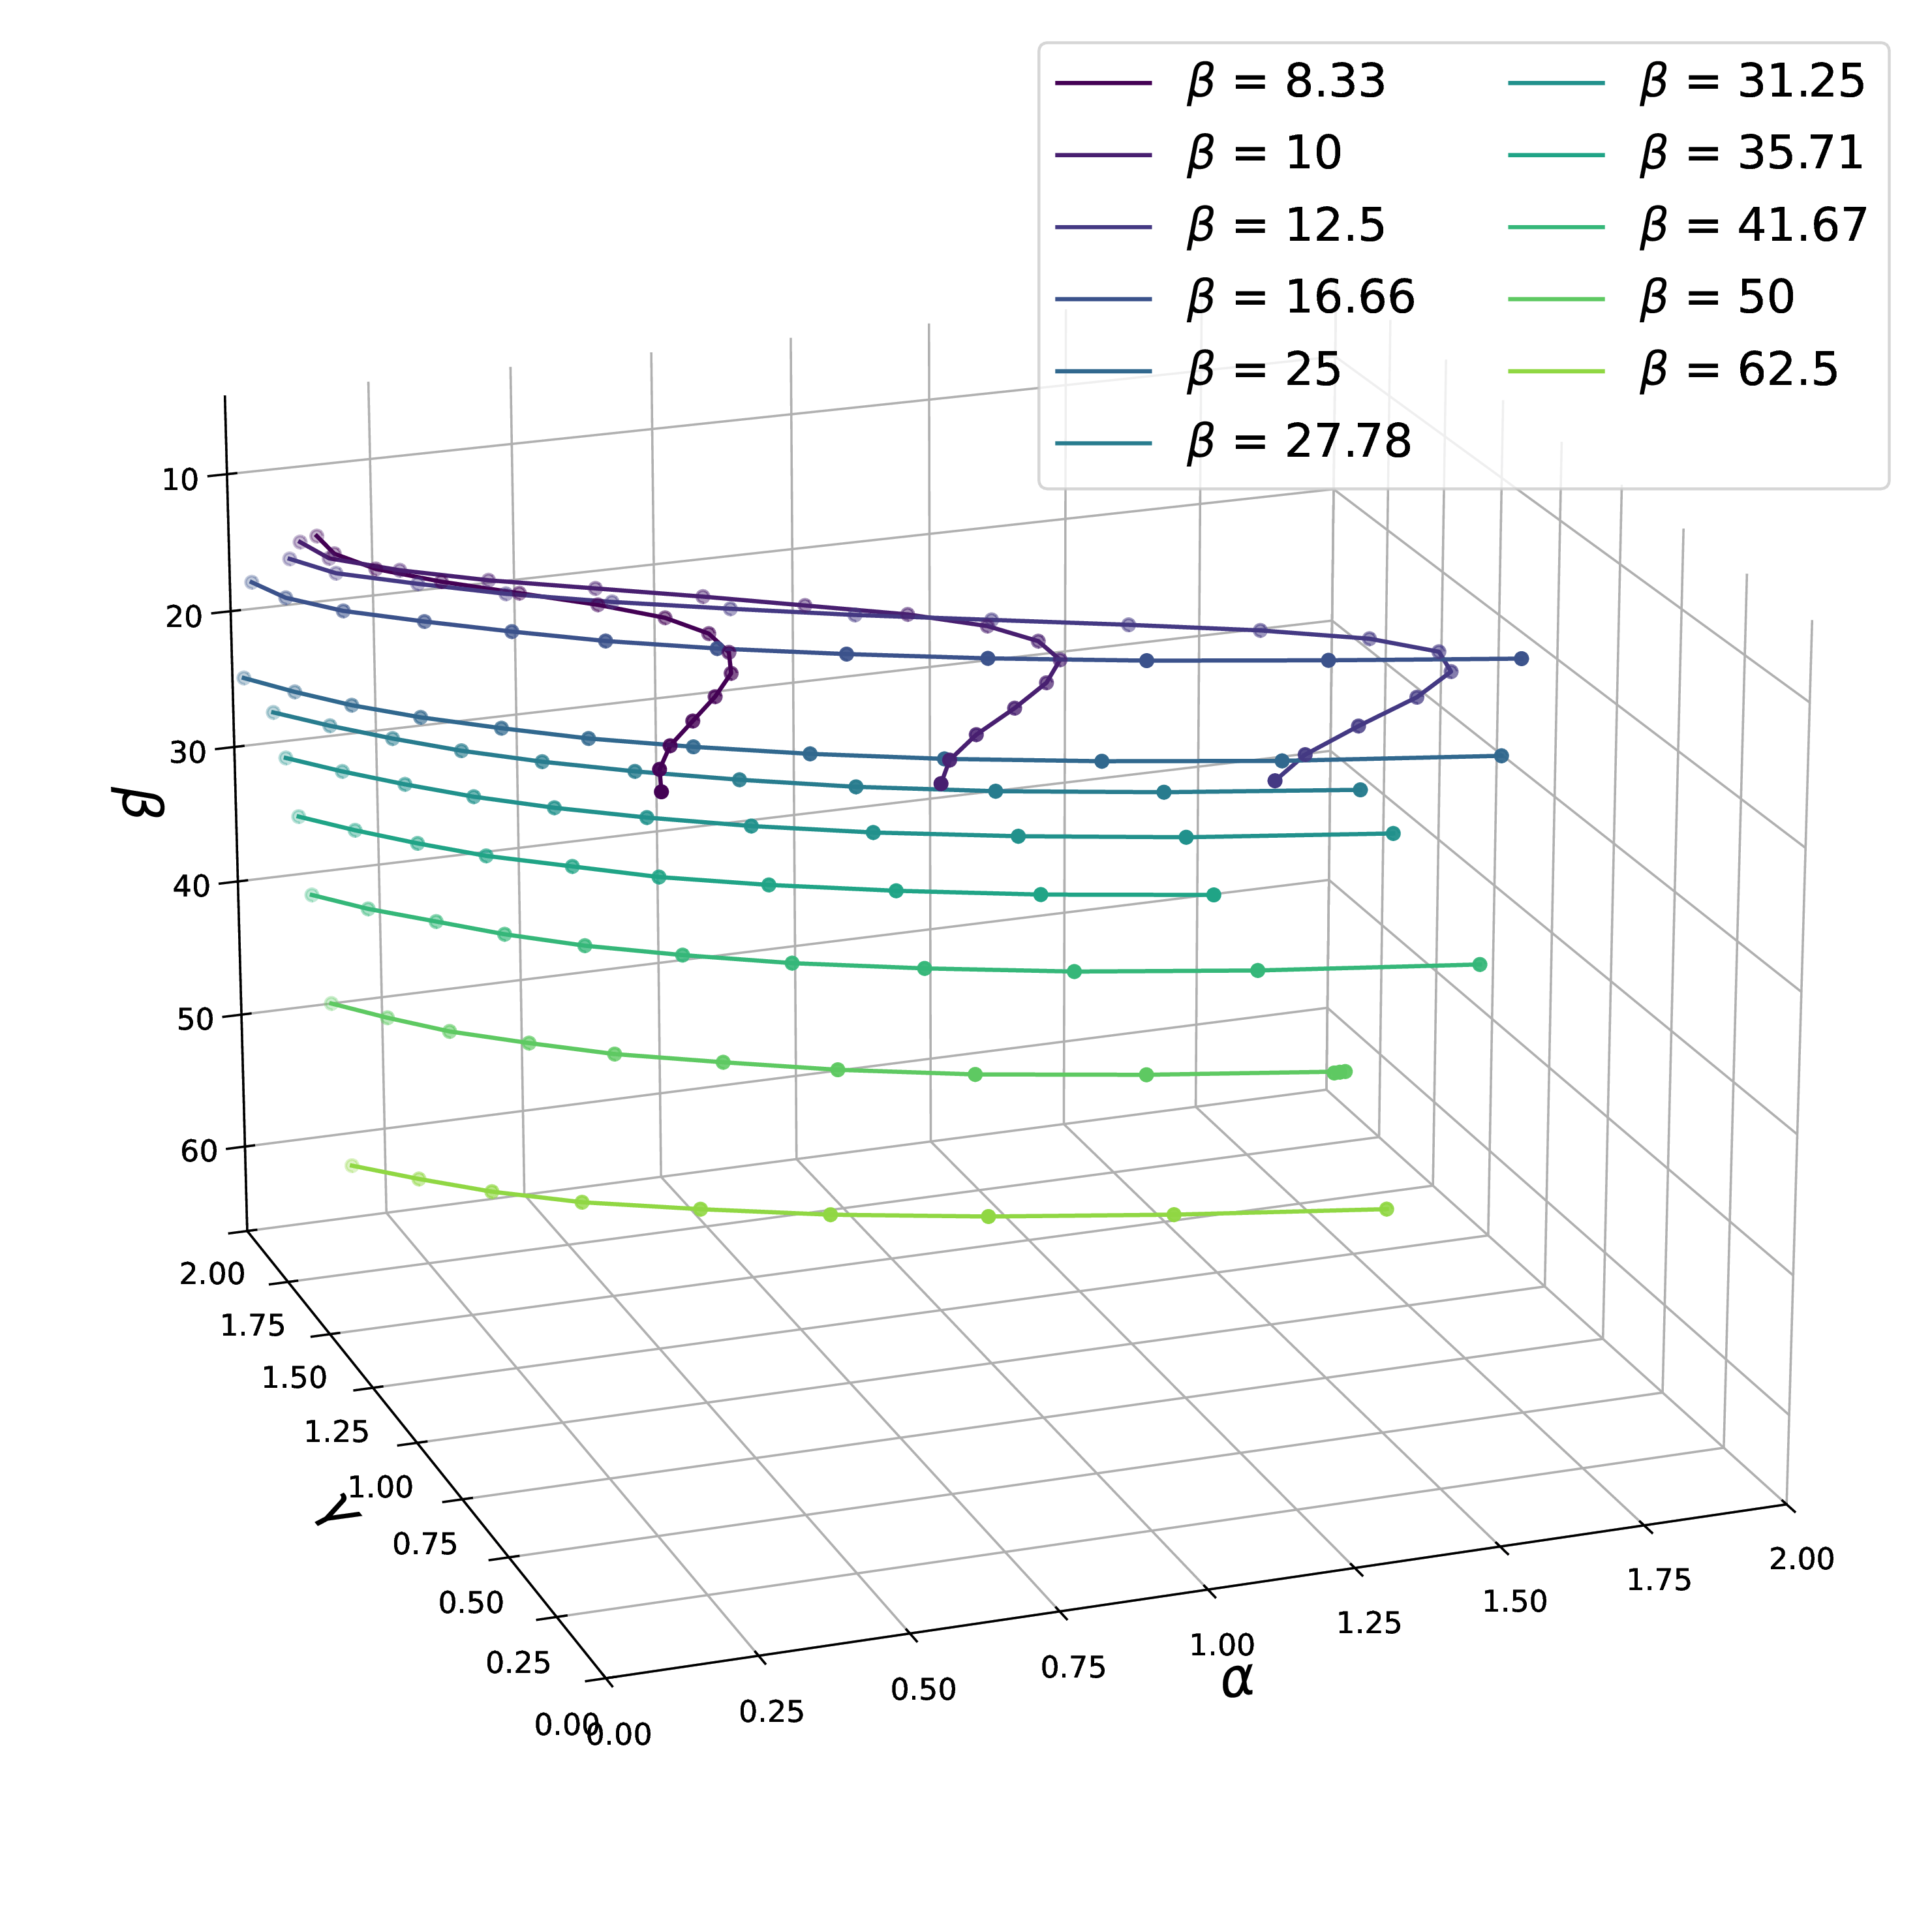
\includegraphics[width=9cm]{TexFigure/3dplot_Ns3_proj_n (0).png}}
  \caption{3-Dimension plotting of upper Figure, Fig.17,  with $\beta$ axis}
\end{figure}

\begin{figure}[htbp]
  \centerline{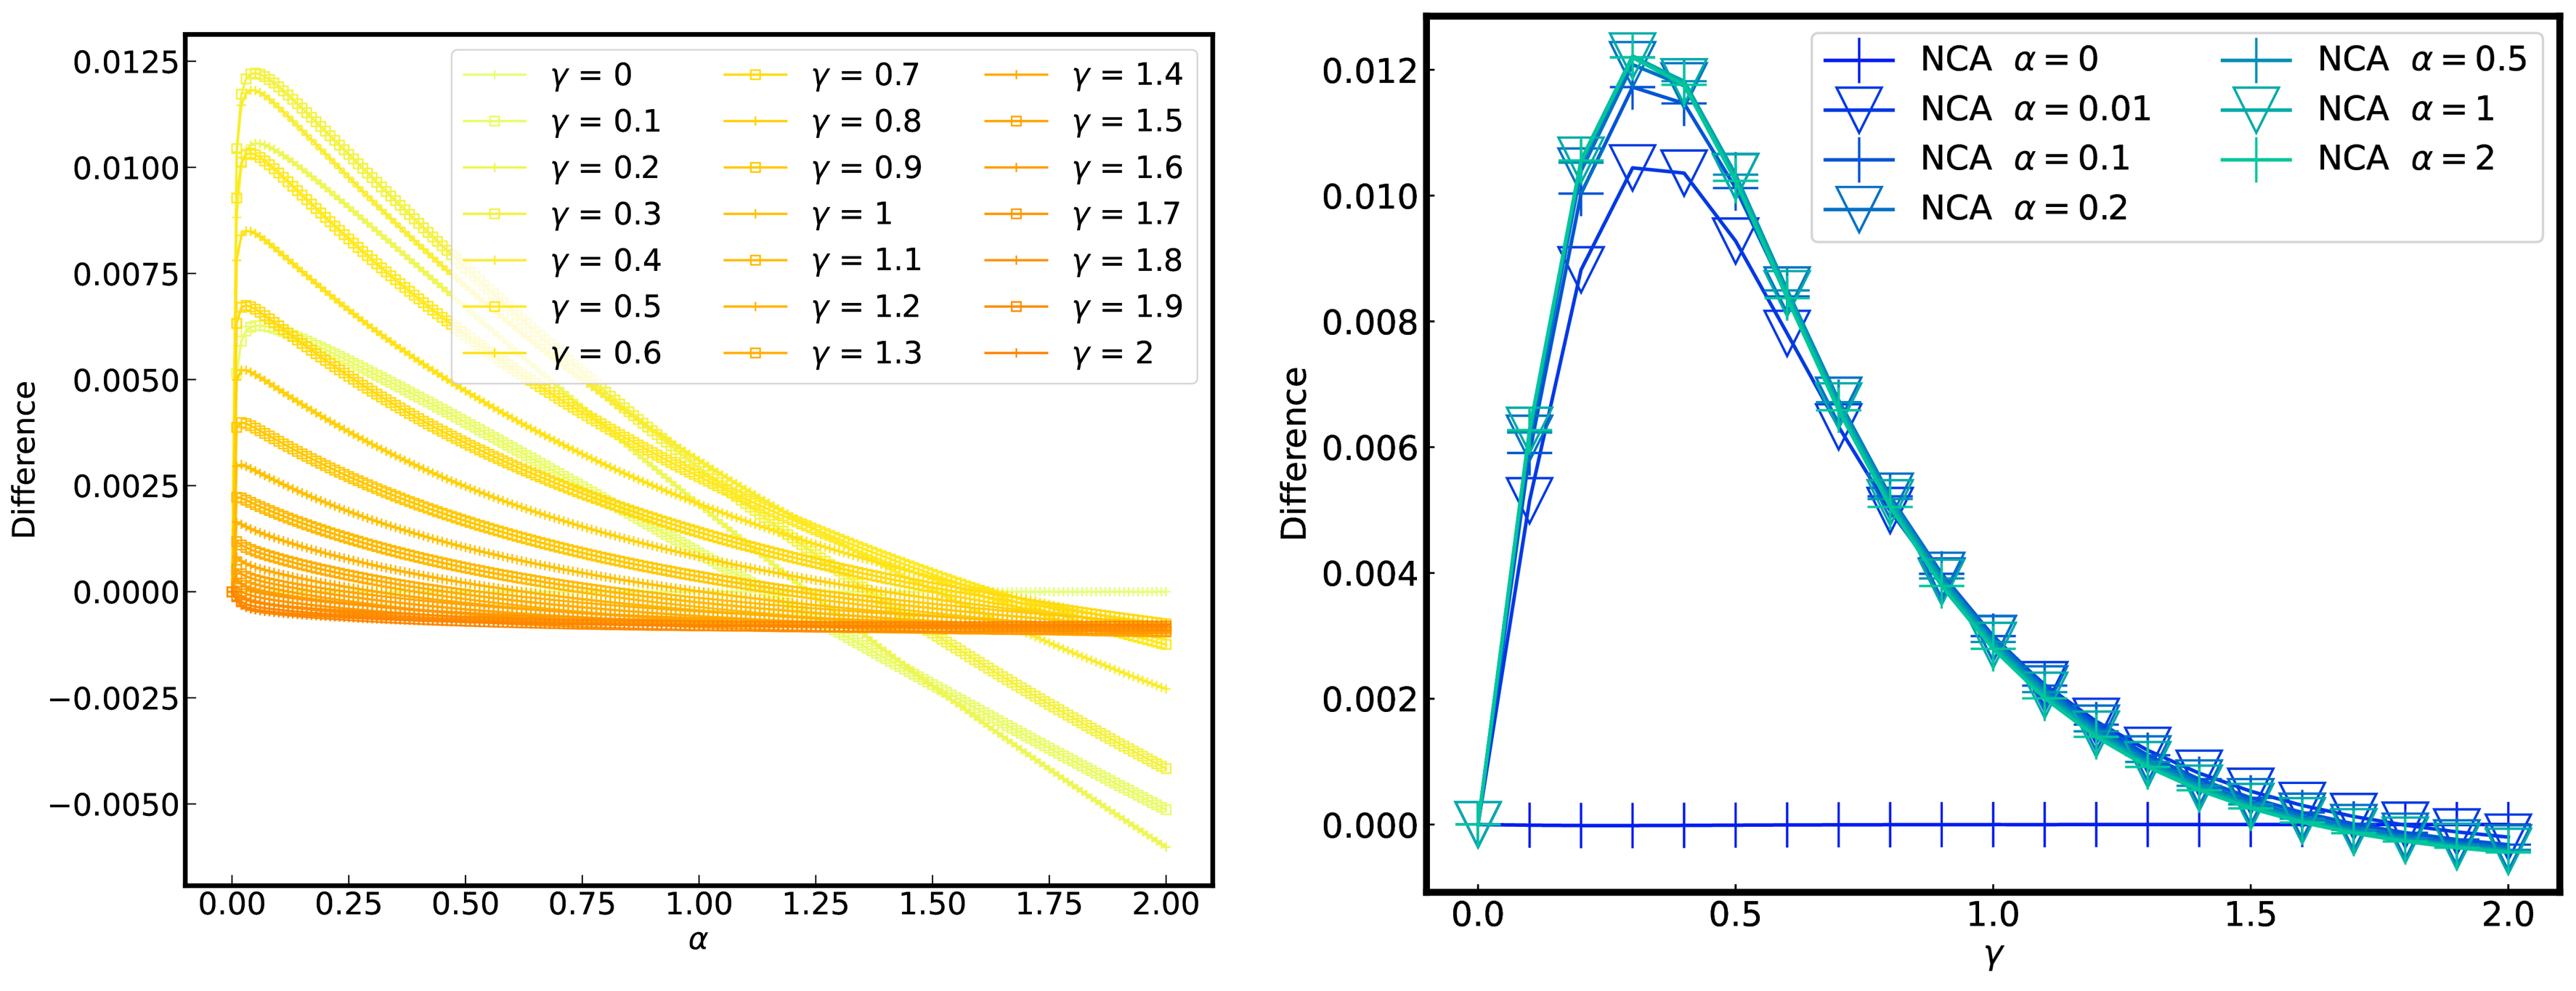
\includegraphics[width=12cm]{TexFigure/swap_fig.png}}
  \caption{The crossing picture in $\alpha$ swapping, $\gamma$ swapping}
\end{figure}
\pagebreak
\section*{5.5 $\chi_{sp}$}
Calculating the phase transition using the relationship between the correlation function and the DC conductivity, 
we observed the following results: Varying the $\gamma$ value at a fixed $\alpha$ value, 
conductivity tended to decrease as the interaction with the external environment increased. 
In particular, at low temperatures, the conductivity increased up to a certain value
while the rate of change decreased with respect to the $\alpha $ value. \\
When we fixed the $\gamma$ value and varied the $\alpha$ value, the conductivity always increased at high temperatures. 
However, at low temperatures, we observed that the conductivity decreased as the $\alpha$ value increased.
\begin{figure}[htbp]
  \centerline{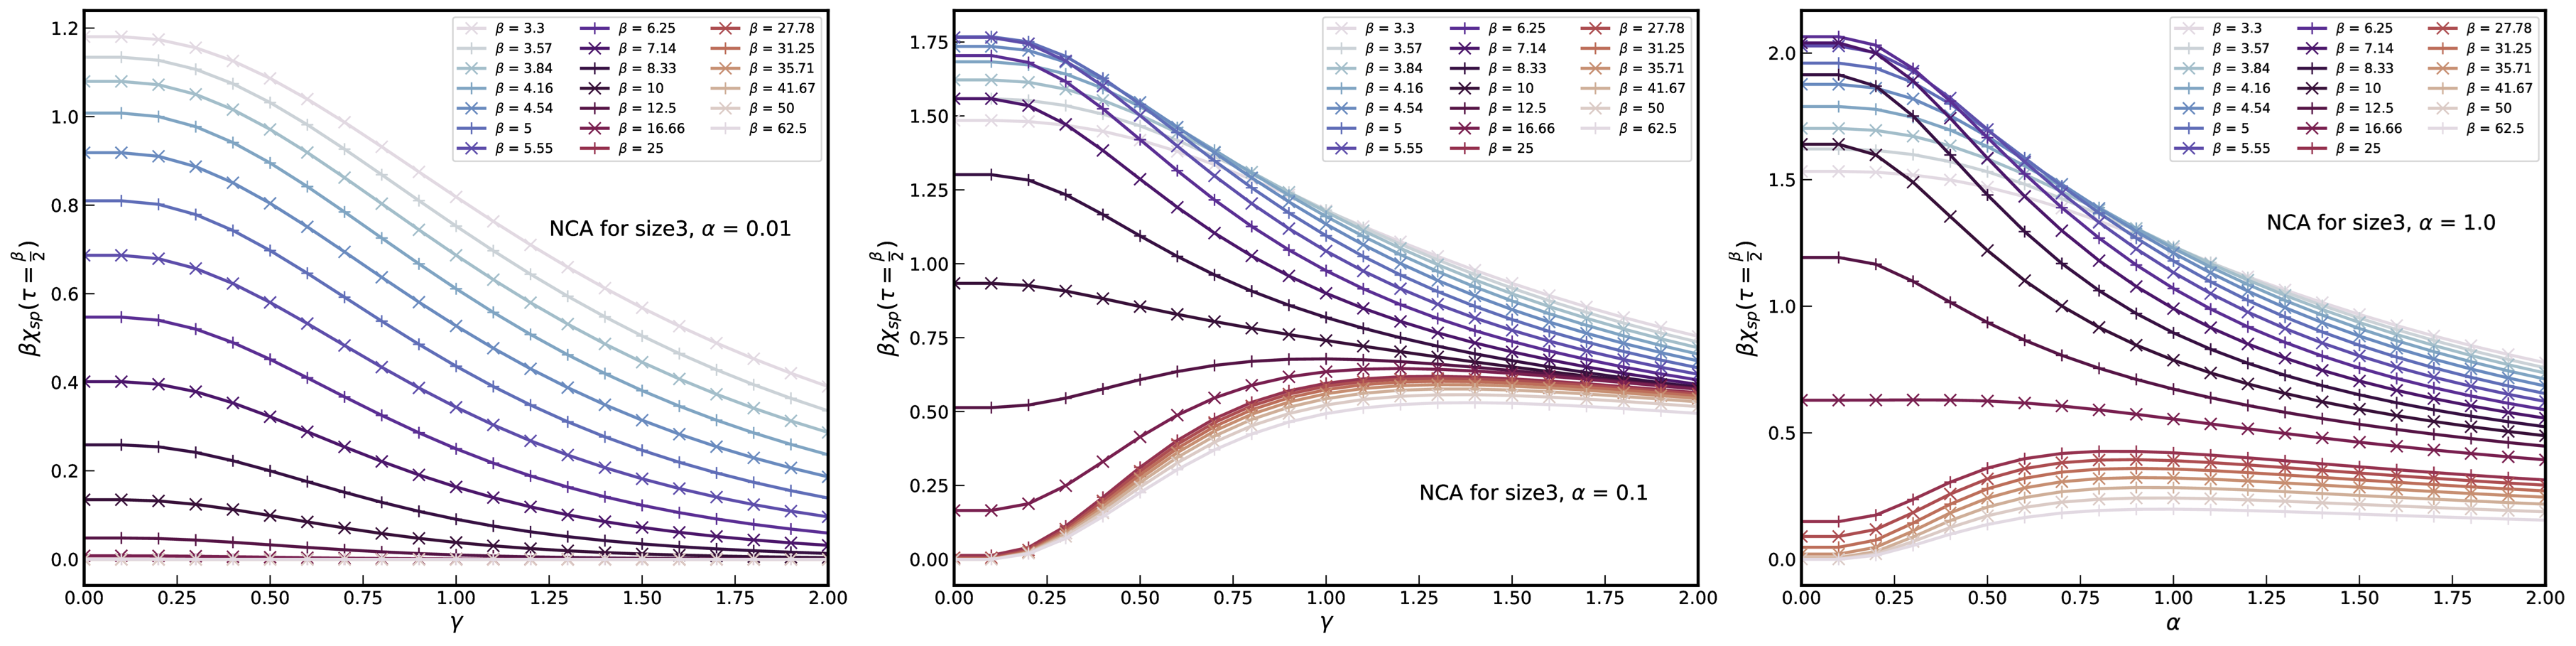
\includegraphics[width=14cm]{TexFigure/chi_gam_swp.png}}
  \centerline{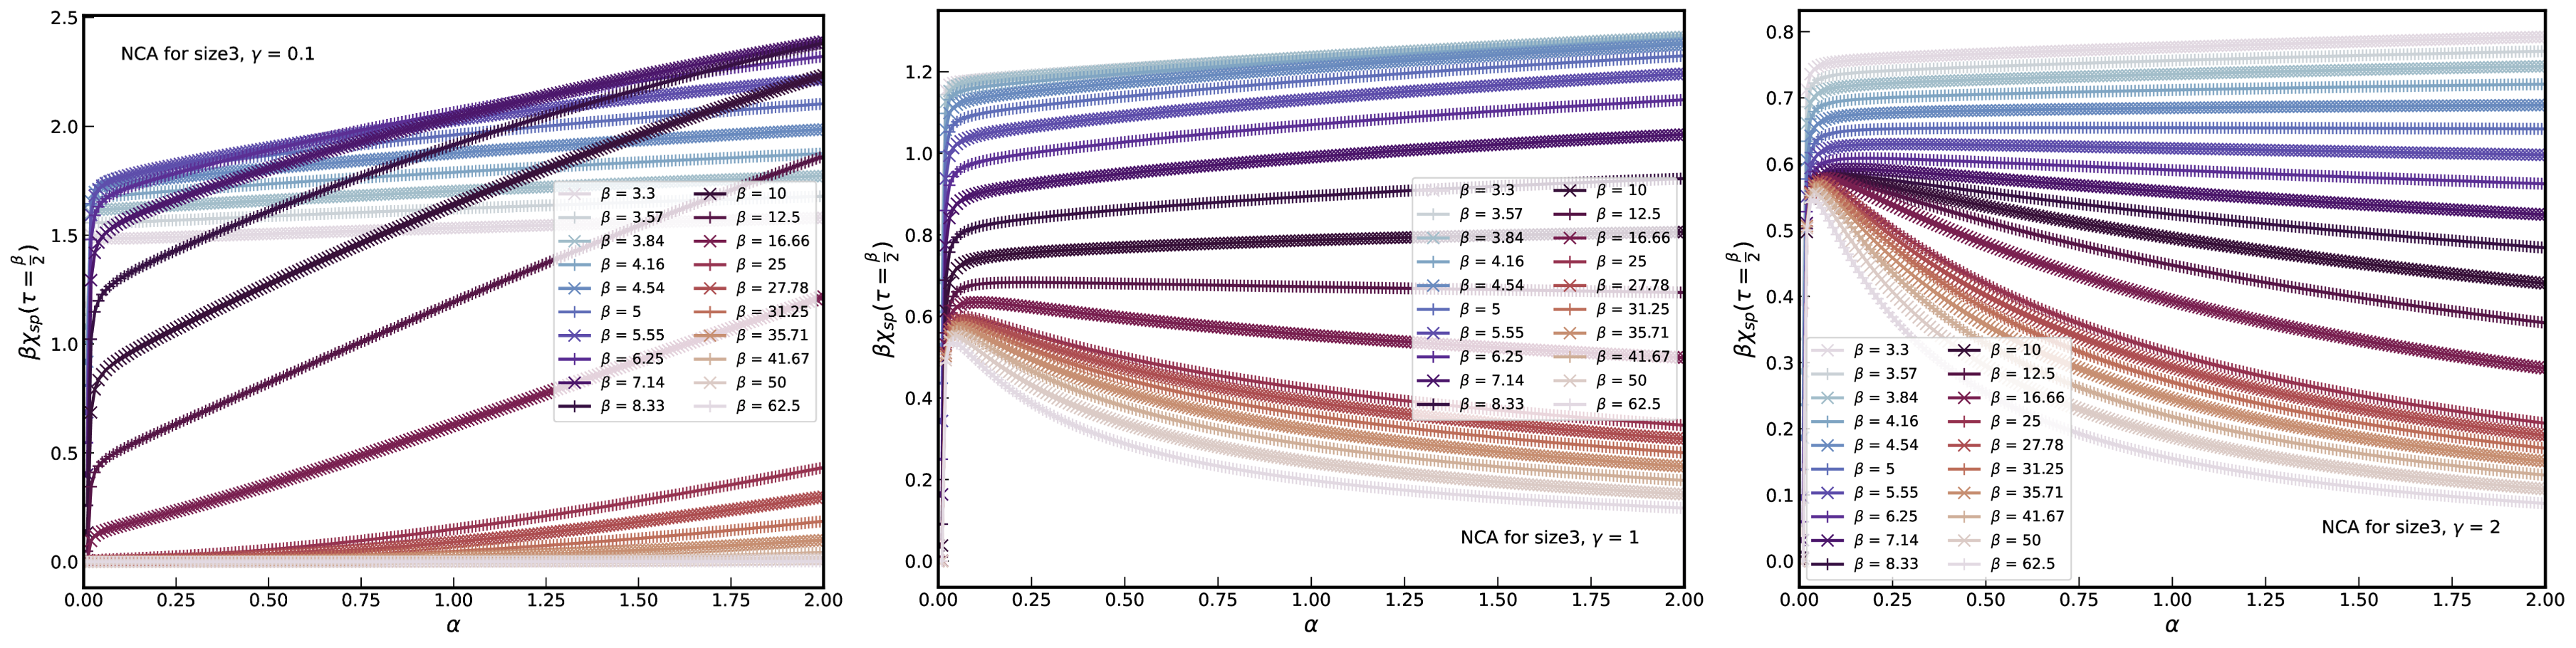
\includegraphics[width=14cm]{TexFigure/chi_alp_swp.png}}
  \caption{The crossing picture in $\chi_{sp}$ with $\gamma$ swapping and $\alpha$ swapping}
\end{figure}
To observe how the conductivity changes for all $\gamma$ and $\alpha$ value conditions at a fixed temperature, 
we visualized the results using a 2D color map. At high temperatures, 
we observed that the conductivity increased as the $\gamma$ and $\alpha$ values increased. 
At low temperatures, the conductivity generally decreased as the influence of the external environment increased. 
Yet the junction energy increased, conductivity tended to increase in stronger influence from the external environment.
\begin{figure}[htbp]
  \centerline{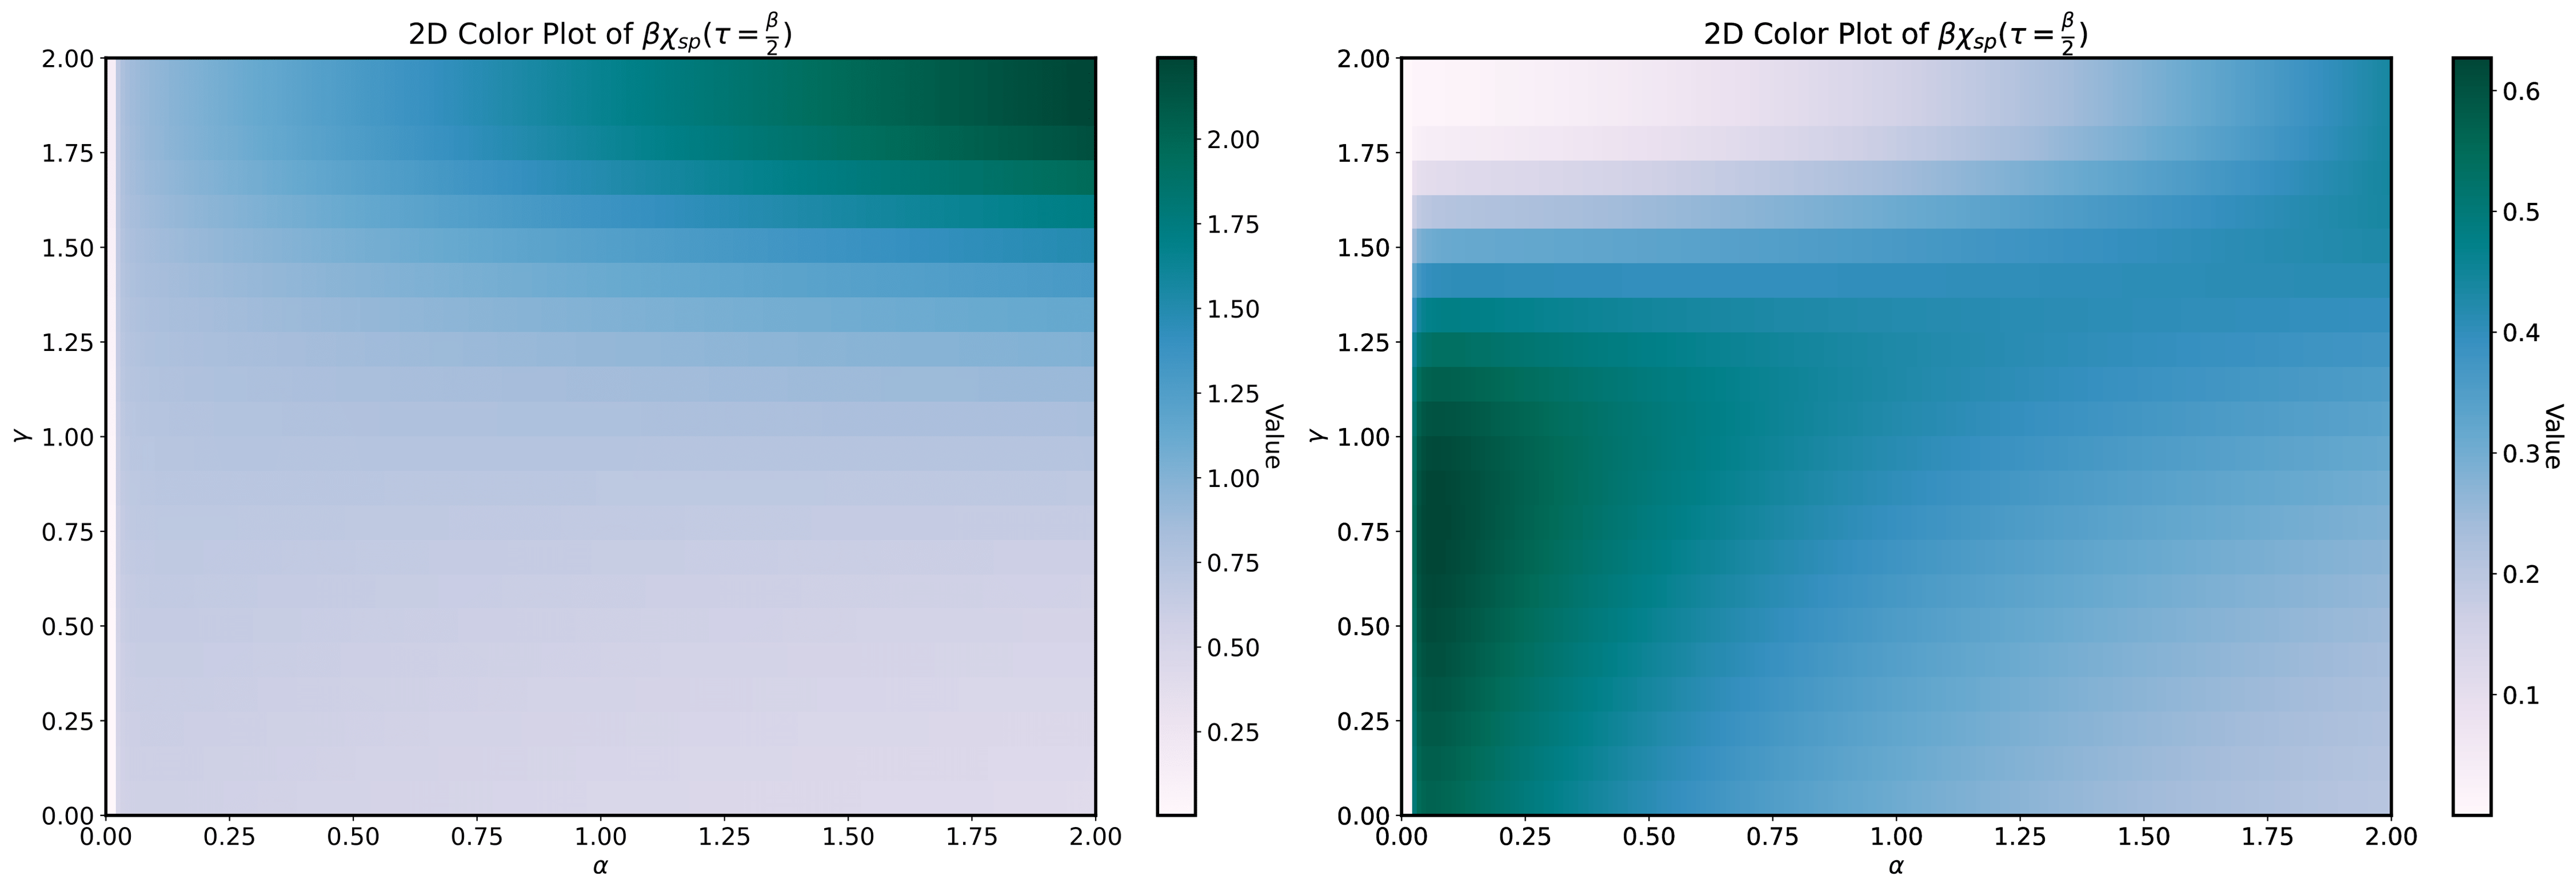
\includegraphics[width=16cm]{TexFigure/chi_color.png}}
  \caption{Colored plot for DC conductivity approximation. Left figure is in $\beta=10$, Right is for $\beta=25$.}
\end{figure}
\end{spacing}

\pagebreak
\newpage

\end{document}